\documentclass[10pt, twoside]{article}   	% use "amsart" instead of "article" for AMSLaTeX format
% Reference https://www.overleaf.com/learn/latex/How_to_Write_a_Thesis_in_LaTeX_(Part_3):_Figures,_Subfigures_and_Tables
%-------------------------------------------------------%
%% packages
\usepackage{graphicx}				% Use pdf, png, jpg, or eps§ with pdflatex; use eps in DVI mode
\graphicspath{{figures/}} % Define the graphicspath
\usepackage{caption} %subfigure
\usepackage{subcaption}%subfigure
\usepackage{stackengine} %add source
%\usepackage{wrapfig} % wrap around a pic 
\usepackage{float}%Force figure placement in text, the default behaviour of figures is to float, so that LaTeX can find the best way to arrange them in your document and make it look better.
\usepackage{fullpage}	
							% TeX will automatically convert eps --> pdf in pdflatex
\usepackage{amssymb}
\renewcommand{\baselinestretch}{1.5}
\usepackage{url}
\PassOptionsToPackage{hyphens}{url}\usepackage{hyperref}   % forcing linebreaks in \url
\usepackage
[
        a4paper,% other options: a3paper, a5paper, etc
        left=2.5cm,
        right=2.5cm,
        top=2cm,
        bottom=3cm,
        % use vmargin=2cm to make vertical margins equal to 2cm.
        % us  hmargin=3cm to make horizontal margins equal to 3cm.
        % use margin=3cm to make all margins  equal to 3cm.
]
{geometry}
%-------------------------------------------------------%
%package for inserting cod %
\usepackage{listings} 
\lstset{frame=tb,
  language=Java,
  aboveskip=3mm,
  belowskip=3mm,
  showstringspaces=false,
  columns=flexible,
  basicstyle={\small\ttfamily},
  numbers=none,
  numberstyle=\tiny\color{gray},
  keywordstyle=\color{blue},
  commentstyle=\color{jo},
  stringstyle=\color{mauve},
  breaklines=true,
  breakatwhitespace=true,
  tabsize=3
}
%%
%-------------------------------------------------------%
% A beautiful title page
%-------------------------------------------------------%
\usepackage{xcolor}
\definecolor{titlepagecolor}{cmyk}{1,.60,0,.40}
\definecolor{namecolor}{cmyk}{0,0,3,.0} 
%-------------------------------------------------------%
\begin{document}%preamble
%-------------------------------------------------------%
\begin{titlepage}
\newgeometry{left=7.5cm} %defines the geometry for the titlepage
\pagecolor{titlepagecolor}
\noindent
\color{white}
\makebox[0pt][l]{\rule{1.3\textwidth}{1pt}}
\par
\noindent
\LARGE {\textbf{\textsf{Manage Your Health Data}} \textcolor{namecolor}{\textsf{ | EIT Health}}}
\vfill
\noindent
{\huge \textsf{DJ's Notes}}
\vskip\baselineskip
\noindent
\textsf{2019}
\end{titlepage}
\restoregeometry % restores the geometry
\nopagecolor% Use this to restore the color pages to white
% ----------------------------------------------------------------

\raggedbottom

\newpage
\tableofcontents %% Content
\vfill
\noindent
\listoffigures
\vfill
\noindent
\textbf{Course Link} \url{https://www.futurelearn.com/courses/managing-your-health-data} 
%-------------------------------------------------------%
%-------------------------------------------------------%
%%Template
\pagebreak
\section{Week 1: What is healthcare data?}
\subsection{Health data}
\begin{enumerate}
\item \textbf{What is data?} Facts and statistics collected together for a reference or analysis. Data is the basic platform to get information. 
\item \textbf{What is information?} The result obtained after the data analysis
\item \textbf{What is health data?}  All the data related to health conditions, laboratory results, metrics and medical research, is known as clinical or health data.
\item \textbf{Who generates the health data?} Hospitals, medical organizations, pharmacies and citizens... they all generate data. 
\item \textbf{What is health data used for?} The main purpose of collecting health data is to store the information related to a patient. The data is also used for research, clinical trials or in some cases billing.
\item \textbf{Why should we manage our healthcare data?} Dietary habits, physical exercise, activity logs, self-generated observations, and other types of lifestyle information can have \textbf{a significant impact on our clinical care and can influence decisions healthcare professionals make about our health}. To exploit such data, citizens must adopt a more proactive role and become essential players in managing their own health data.
\end {enumerate}
%-------------------------------------------------------%
%-------------------------------------------------------%
%-------------------------------------------------------%
%-------------------------------------------------------%
\subsection{Electronic Health Records}
\begin{enumerate}
    \item \textbf{What is EHR?} EHR is defined as a digital repository of patient data that is stored and exchanged securely in hospitals. 
    \item \textbf{Who can access EHR?} Storing, managing and analysing patient data in the EHRs can be accessed by both physicians and patients anytime when required and using a secure online system.
    \item \textbf{Why is EHR useful?}  EHRs can store data securely and track a patient’s health over time. As they are digital they are searchable, so reduces time and the need for duplicate records.
\end {enumerate}
%-------------------------------------------------------%
%-------------------------------------------------------%
\subsection{e-Prescriptions }
\begin{enumerate}
%-------------------------------------------------------%
\item \textbf{What is e-prescription used?}
    \begin{enumerate}
        \item Electronic medical prescriptions aims to facilitate the \textbf{management} of patients' health data, 
        \item whilst also ensuring the whole process of prescribing is \textbf{secure}. 
    \end{enumerate}
%-------------------------------------------------------%    
   \item \textbf{How does e-prescription work?}
    \begin{enumerate}
        \item When a clinician prescribed medication to a patient, that prescription is registered in \textbf{a central system in a country}.         
         \item Patient then goes to a pharmacy to pick up his prescribed medication, he uses his health identity card as ID and the pharmacist then accesses the electronic prescriptions that have been assigned to that patient.
     \end{enumerate}
 %-------------------------------------------------------%
\item \textbf{What are the benefits of e-prescription?}
    \begin{enumerate}
        \item Commodity of patients (ease of use for patients)
        \item avoiding duplicate prescriptions
        \item enabling repeat prescriptions to chronic patients
        \item empowering the authentication of prescription dispenses
    \end{enumerate}    
%-------------------------------------------------------%
\end {enumerate}
%-------------------------------------------------------%
%-------------------------------------------------------%
%-------------------------------------------------------%  
%-------------------------------------------------------%


%-------------------------------------------------------%     
%insert a figure
\begin{figure}
   \centering
    %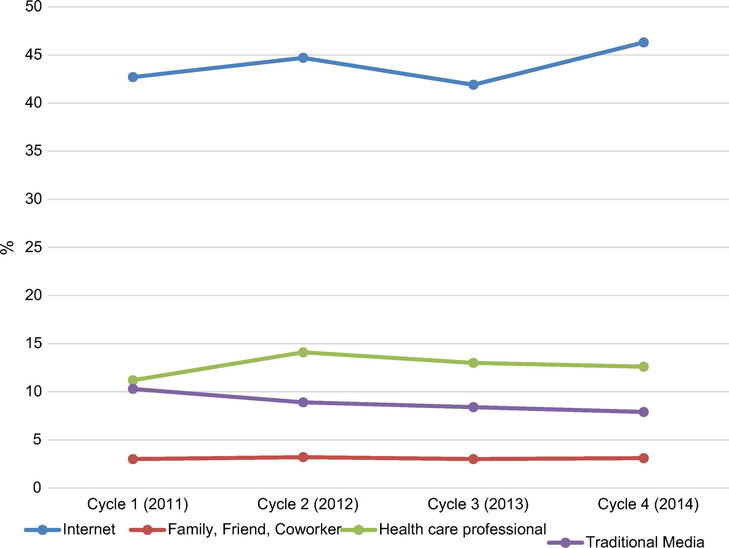
\includegraphics[width=5in]{internet_health.jpeg}%name of the image
      \stackunder{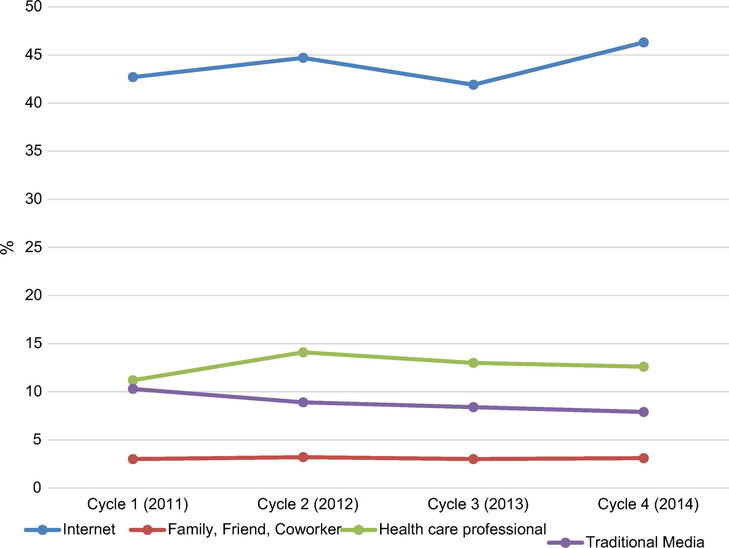
\includegraphics[width=0.8\textwidth]{internet_health.jpeg}}%
             {\scriptsize%
             Source: \url{https://www.tandfonline.com/doi/figure/10.1080/23311886.2017.1302785?scroll=top&needAccess=true&}}
  \caption{Where patients sought health information first}
  \label{fig:internet_health}
\end{figure}
     %iend of a figure
%-------------------------------------------------------%
%-------------------------------------------------------%
%-------------------------------------------------------%

\section{Week 2: Devices, Apps, and websites with health information }
%-------------------------------------------------------%
%-------------------------------------------------------%
\subsection{Trustworthy Websites with Health Information}
\begin{enumerate}
%-------------------------------------------------------%
\item \textbf{Clinical Information over Internet }
    \begin{enumerate}
        \item \textbf{Patient empowerment} is an essential concept in the latest approach in healthcare. This a concept related to health literacy and the quality of information available for patients.
        \item When asked how important they considered Internet as source of health information, \textbf{ around half of the users} reported to be important or very important.
        \item \textbf{What kind of information do patients need} We need sources of information adapted for patients but curated by health professionals. Always taking into account that health professionals should be our main source of information in relation to our health.
        \item \textbf{Fact from fiction - Who can we trust?} What are the alternative sources to clinical institutions to search for information. Websites with health related information intended for patients, and tools to produce and store health data.     
     \end{enumerate}
%-------------------------------------------------------%
\item \textbf{Managing data outside hospital }
    \begin{enumerate}
        \item There is a plethora of information and tools available online that allow us to search, produce and manage data related to our health, outside of our clinical institution.
    \end{enumerate}
%-------------------------------------------------------%
\item \textbf{Self-diagnosis and the internet}
    \end{enumerate}
%-------------------------------------------------------%
%-------------------------------------------------------%
\subsection{Your health data outside the hospital}
    \begin{enumerate}
%-------------------------------------------------------%
        \item \textbf{The expansion of data enrichment }
            \begin{enumerate}
               \item The traditional way of generating and managing health data was through paper records.
               \item Clinical institutions, doctors and other healthcare professionals will always be the cornerstone of our treatment,                                  
                \item Today, we can greatly enrich the data related to our health with wearable devices, mobile apps and other websites or tools.
            \end{enumerate}   
%-------------------------------------------------------%
        \item \textbf{What is wearables?} 
            \begin{enumerate}
               \item Wearables are a technological gadget with a sensor. 
               \item They can monitor 
               \item These gadgets can be connected to smart phones with lots of apps available, that keep a log of your vital signs and physical activities, daily habits, diet, etc.
               \item Information from wearables can be collected at home, at work or as we go about our day. It \textbf{avoids the use of uncomfortable alternatives} and the data is collected 24 hours a day and can be accessed by most citizens.
            \end{enumerate}   
%-------------------------------------------------------%
    \end{enumerate}
%-------------------------------------------------------%
%---------------------------------------------------%%
 \begin{figure}
     \centering
     \begin{subfigure}[b]{0.8\textwidth}
         \centering
         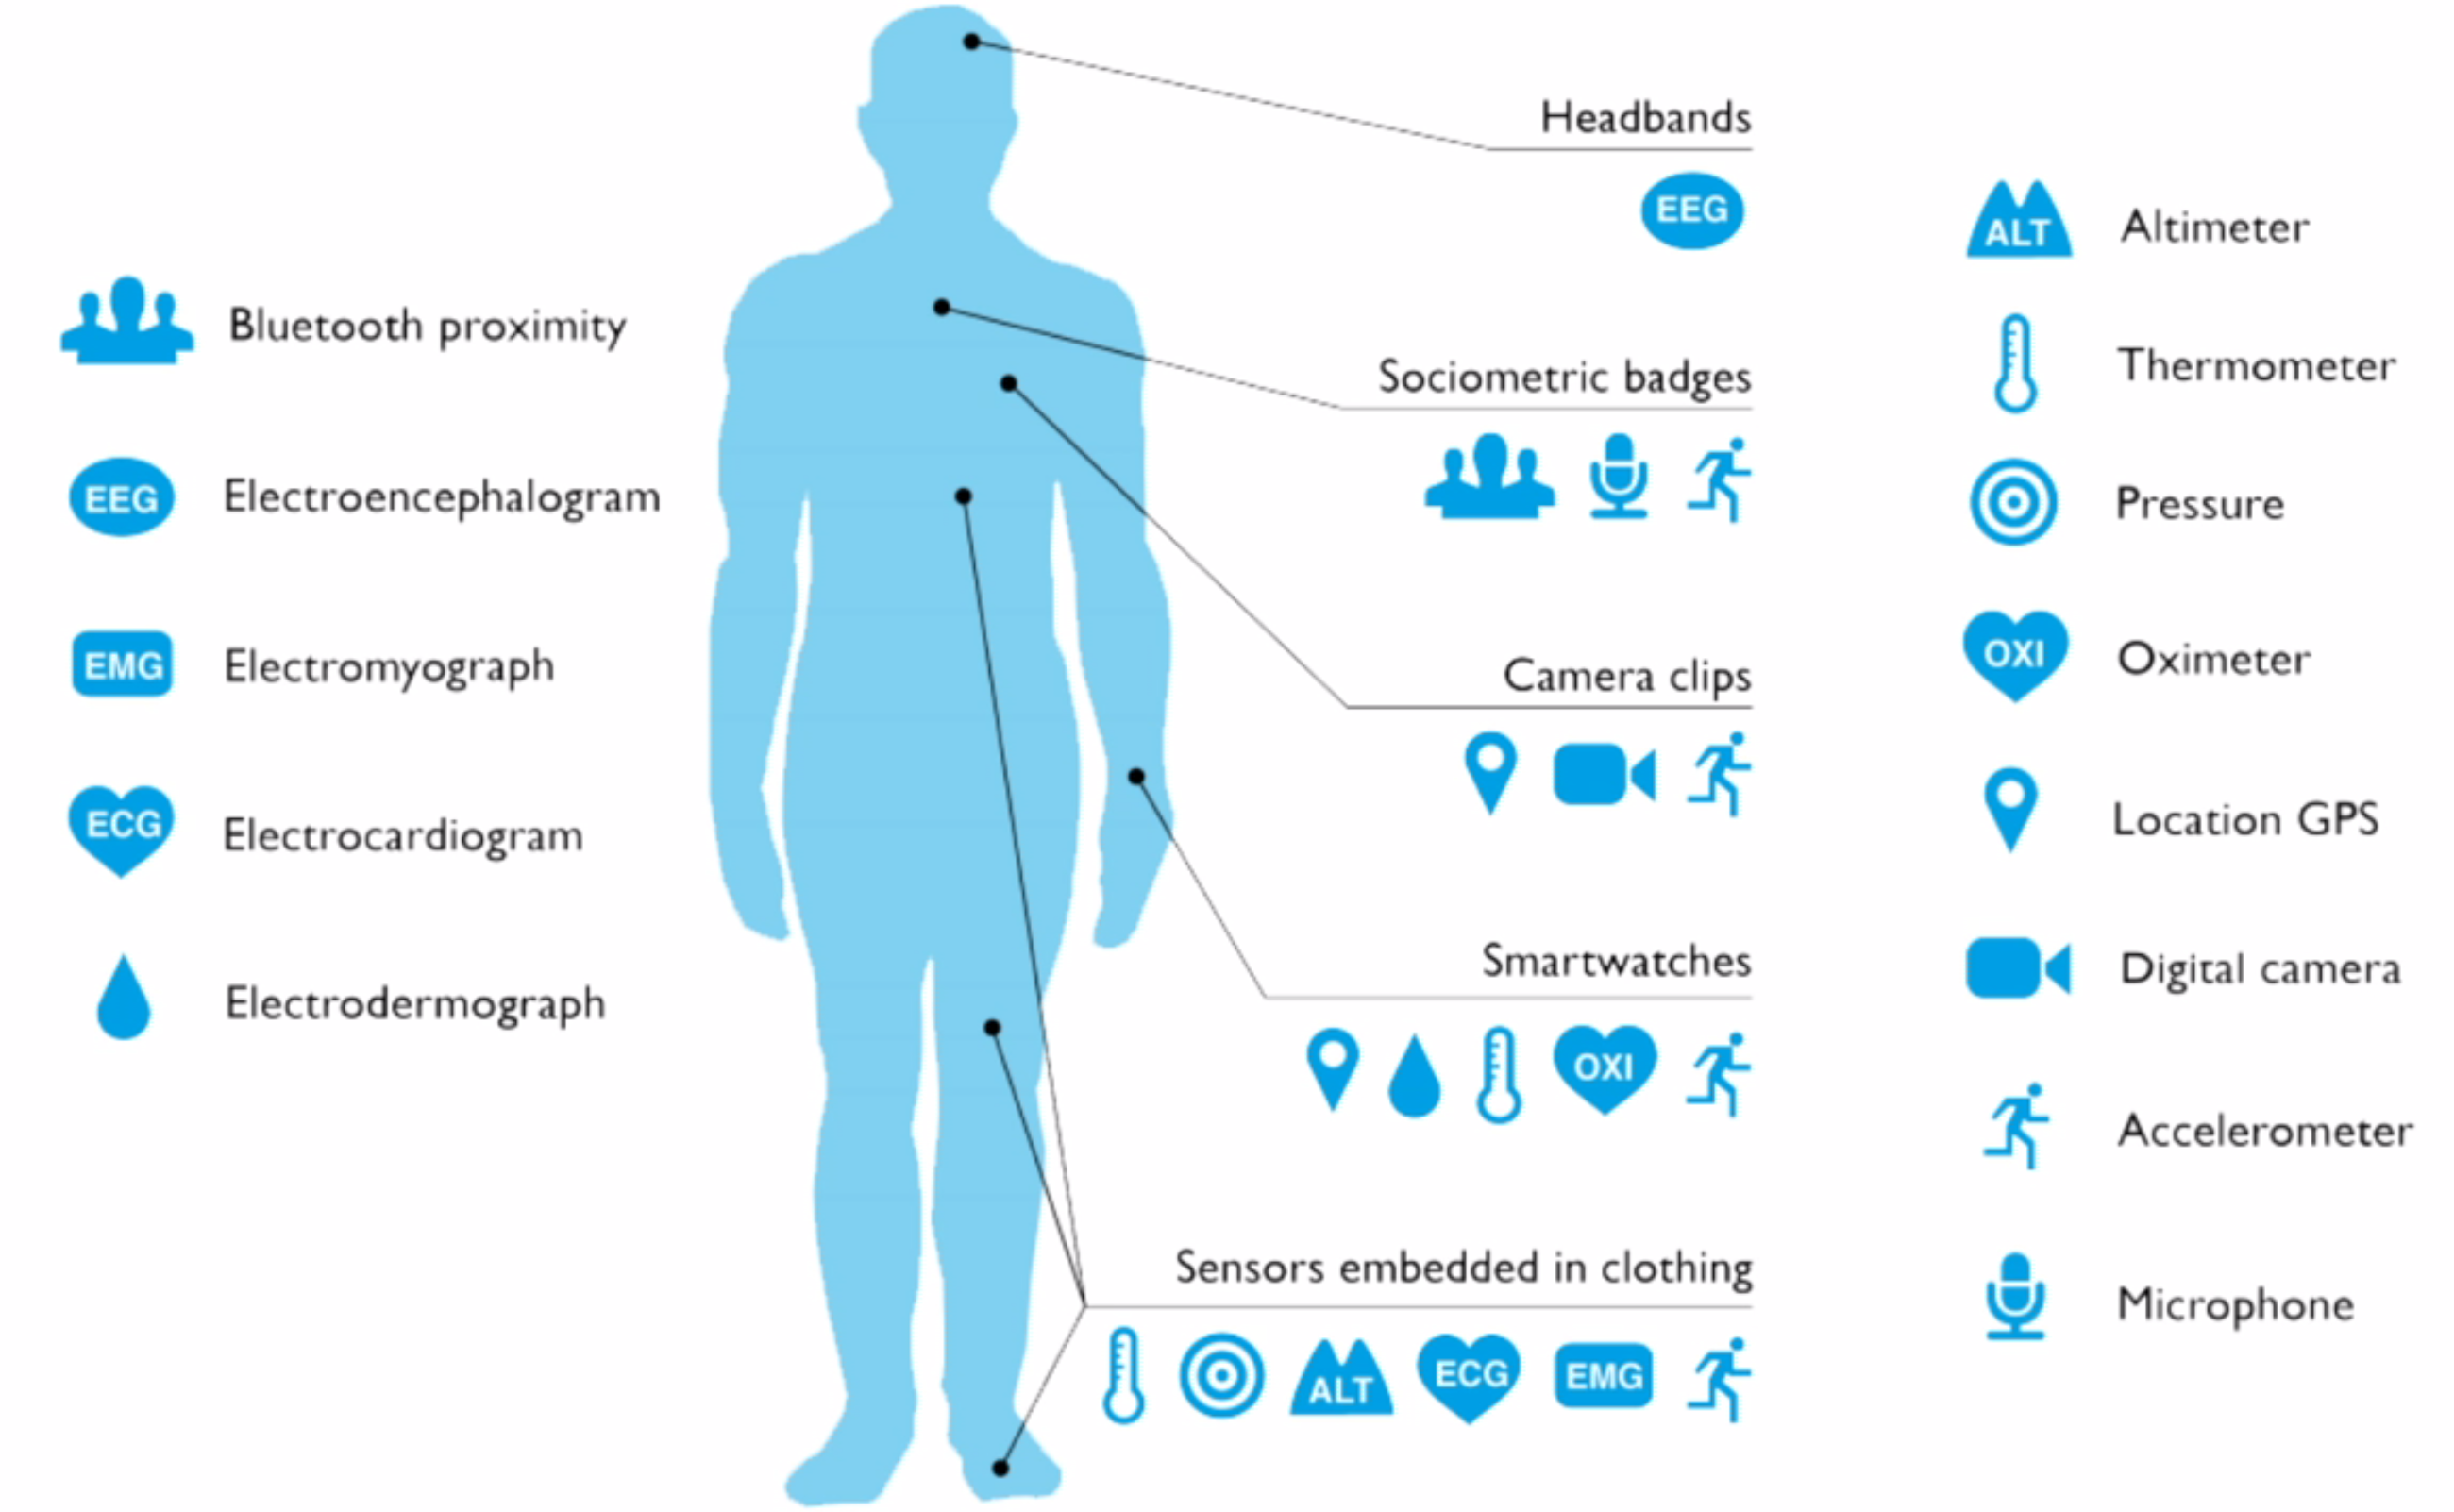
\includegraphics[width=\textwidth]{wearable0.png}
         %\caption{}
         %\label{fig:}
     \end{subfigure}
     \hfill
 %---------------------------------------------------%%
\begin{subfigure}[b]{0.25\textwidth}
    \centering
    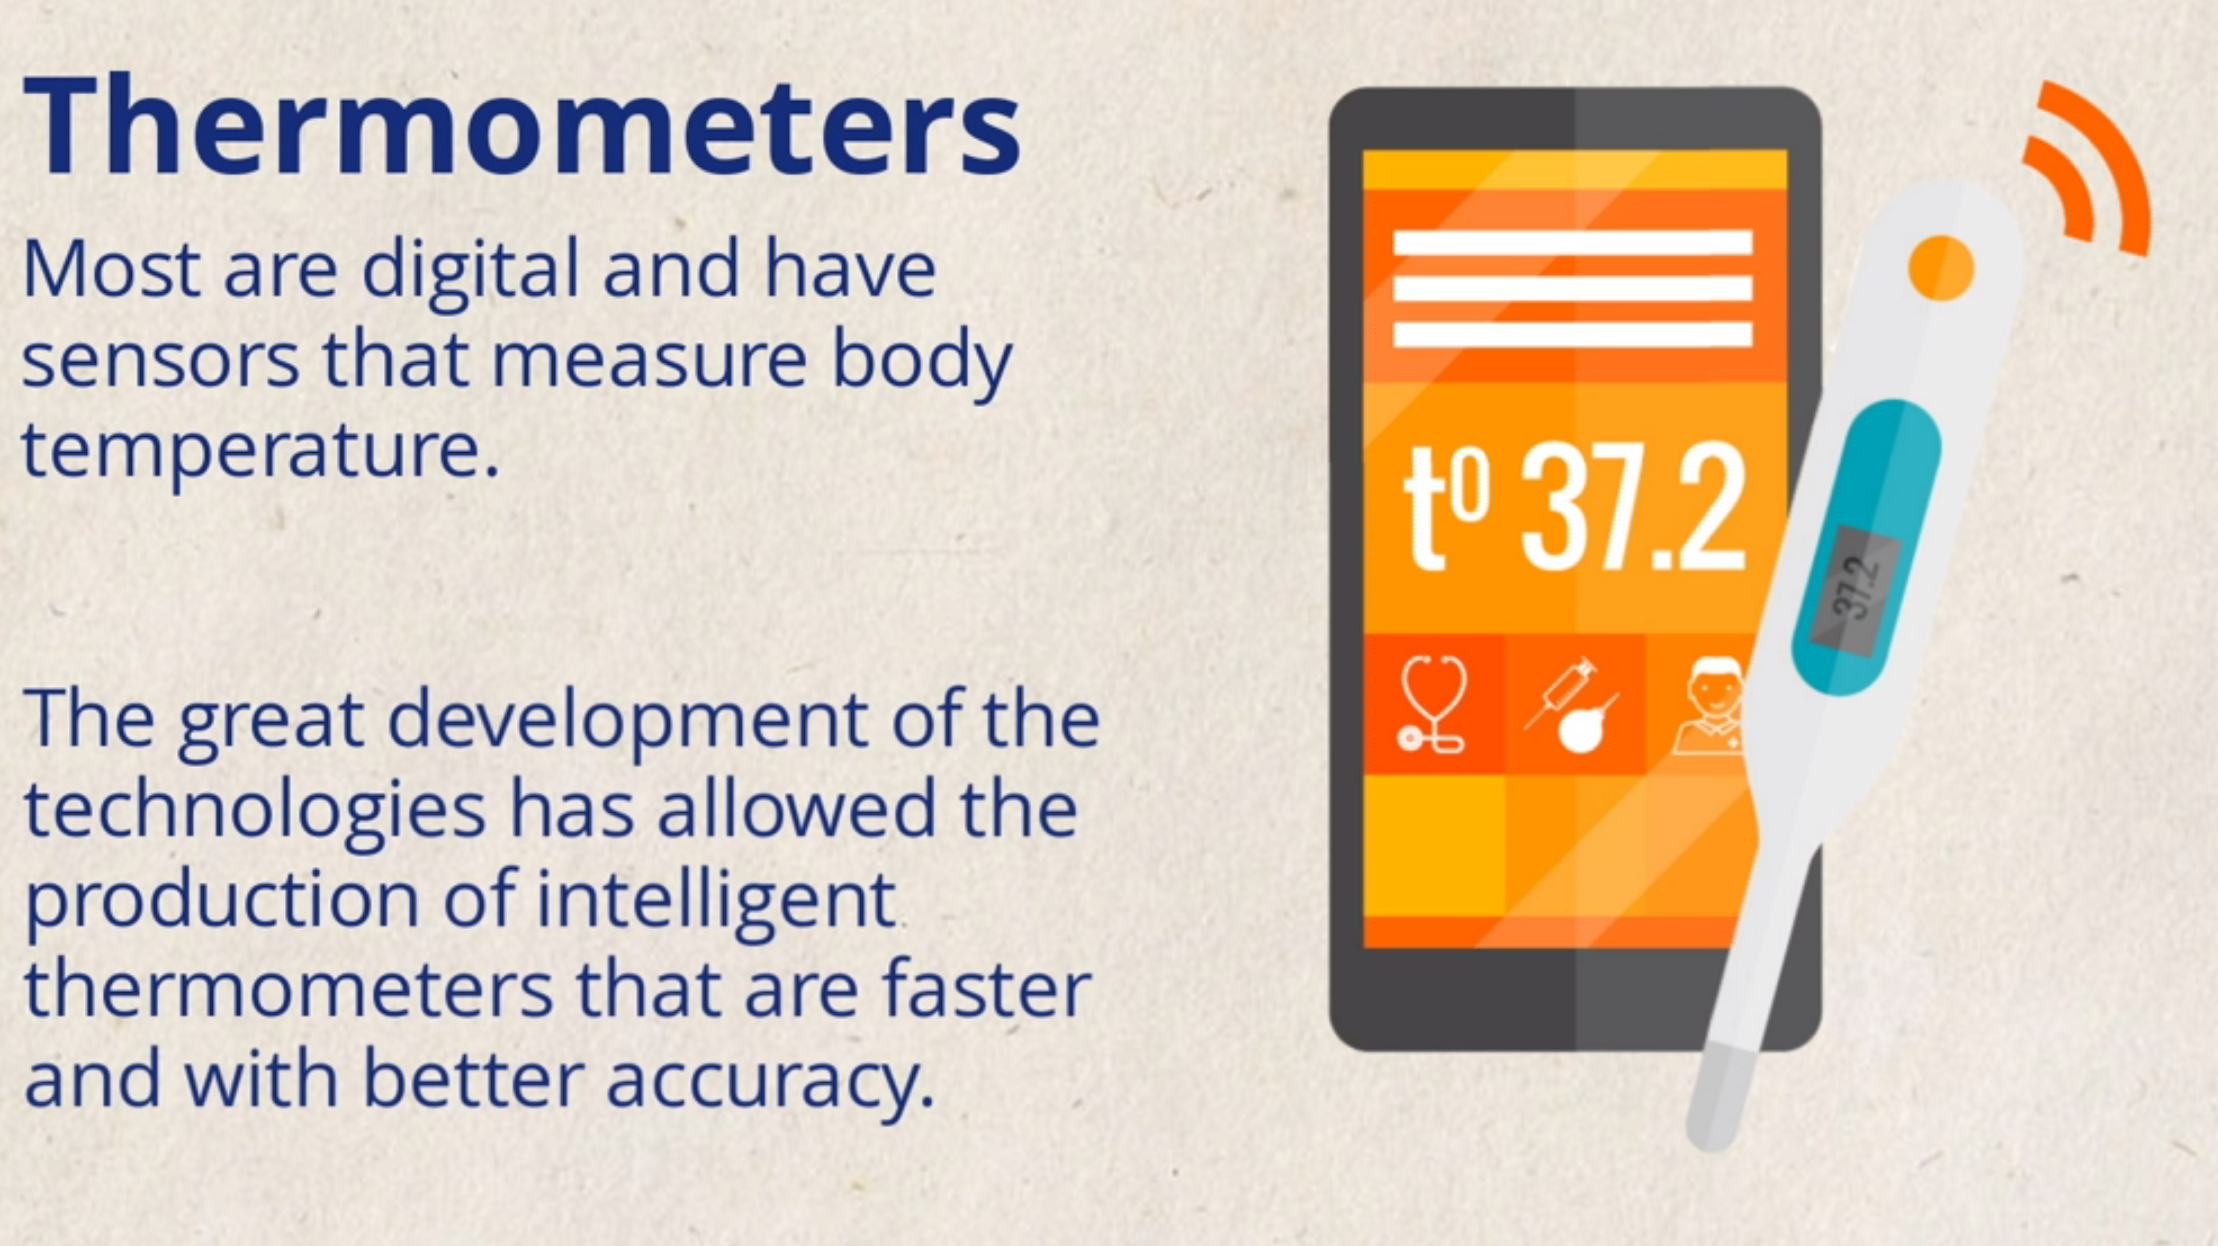
\includegraphics[width=\textwidth]{Thermometer.png}
    %\caption{}
    %\label{fig:}
\end{subfigure}
\hfill
%---------------------------------------------------%%
\begin{subfigure}[b]{0.24\textwidth}
    \centering
    \includegraphics[width=\textwidth]{BloodGlucose.png}
    %\caption{}
    %\label{fig:}
\end{subfigure}
\hfill
%---------------------------------------------------%%
\begin{subfigure}[b]{0.35\textwidth}
    \centering
    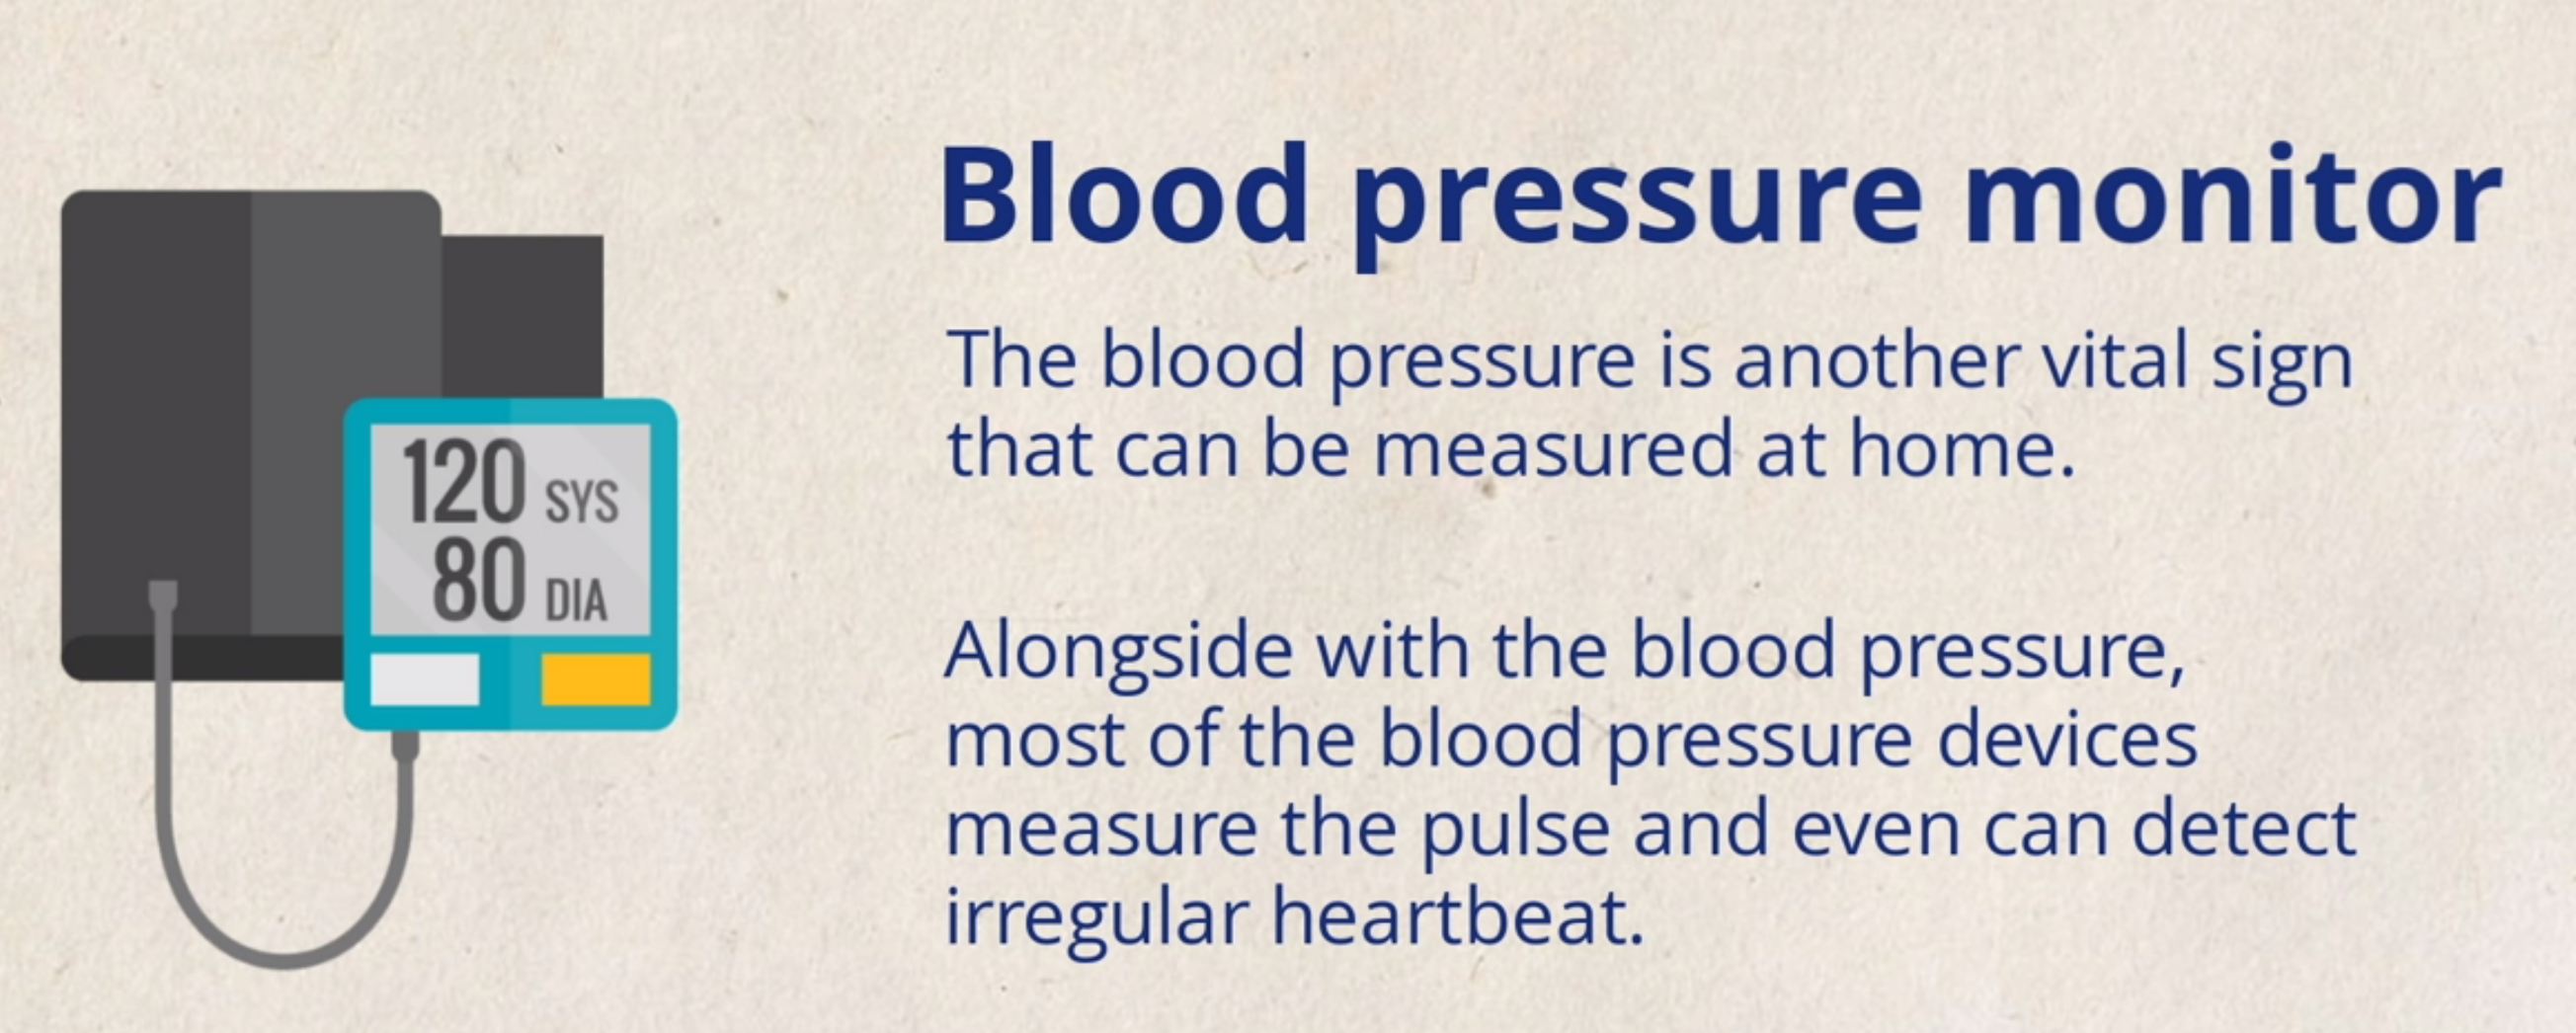
\includegraphics[width=\textwidth]{BloodPressure.png}
    %\caption{}
    %\label{fig:}
\end{subfigure}
\hfill
%---------------------------------------------------%%
%---------------------------------------------------%%
     \begin{subfigure}[b]{0.99\textwidth}
         \centering
         \includegraphics[width=\textwidth]{wearable3.png}
         %\caption{}
         %\label{fig:}
     \end{subfigure}
     \hfill
%---------------------------------------------------%%
\begin{subfigure}[b]{0.45\textwidth}
    \centering
    \includegraphics[width=\textwidth]{wearable1.png}
    %\caption{}
    %\label{fig:}
\end{subfigure}
\hfill
%---------------------------------------------------%%
\begin{subfigure}[b]{0.37\textwidth}
    \centering
    \includegraphics[width=\textwidth]{wearable2.png}
    %\caption{}
    %\label{fig:}
\end{subfigure}
\hfill


%\stackunder{\includegraphics[width=0.8\textwidth]{}}%
             {\scriptsize%
             Source: \url{https://www.futurelearn.com/courses/managing-your-health-data/2/steps/473546}}
  \caption{Wearables}
  \label{fig:Wearables}
\end{figure}
%-------------------------------------------------------%
%-------------------------------------------------------%
%-------------------------------------------------------%
%-------------------------------------------------------%
\pagebreak
\section{Week 3: Self-management of health data - Does it really work?}
%-------------------------------------------------------%
%-------------------------------------------------------%
\subsection{Security, Legal and Ethical issues }
\begin{enumerate}
%-------------------------------------------------------%
\item \textbf{The data protection directive from the EU}
    \begin{enumerate}
       %Daily and rapid generation of clinical data and the development of applications related to healthcare has led to certain considerations about data protection.
        \item \textbf{How is health and genetic data classified?} A special category of data requiring a higher level of data protection
        \item The technology used for clinical data protection and encryption must be taken to the greatest consideration because of the sensitivity of the information. 
        \item \textbf{What issues do we need to consider regarding health data?} 
            \begin{enumerate}    
                \item Security issue
                    \begin{itemize}
                        \item How is our data protected against unauthorized use or modification?
                        \item To protect the data, encryption techniques are used to prevent attacks and access by unauthorized persons.
                    \end{itemize}                                            
                \item Ethics issues 
                    \begin{itemize}
                        \item Concerned with privacy, confidentiality and consent. 
                        \item Data privacy: the private communication between patients and healthcare specialists must be guaranteed and any information about patients must be confidential.
                        \item Confidentiality: any information about a patient must be confidential.
                        \item Consent: collecting and processing patient's data requires their permission.                     
                      \end{itemize}                      
                \item Legal Privacy: All the information about laws and directives to protect individuals' privacy is related to legal issues.
             \end{enumerate}      
        \item \textbf{Sharing your data} 
            \begin{enumerate}    
                \item It is forbidden to share personal data unless the person gives his consent.
                \item If a patient gives permission, then their health data can be processed.
                \item Exceptions:
                    \begin{itemize}
                        \item In case of emergency, no consent is required since sharing health data is vital for the patient.
                        \item It is allowed to share health data between health specialists that are treating the patient.
                        \item Consents forms must be clear and unambiguous for patients.
                    \end{itemize}                            
            \end{enumerate}                
   \end{enumerate}
 \end {enumerate}
 %-------------------------------------------------------%
%-------------------------------------------------------%
\subsection{Health data - Advantages and disadvantages}
\begin{enumerate}
%-------------------------------------------------------%
\item \textbf{Technology - friend or Foe?}
%-------------------------------------------------------%
\item \textbf{Barriers to health data self-management}
    \begin{enumerate}
        \item \textbf{Technology}
            \begin{enumerate}
                \item Barriers come from how data is generated and stored.
                \item EHR clinical data generated in hospitals is coded using different terminologies and formats, depending on the software used. As a consequence, compiling all our health information is not just a matter of putting it in the same place, but also we have to be able to gather it all in the same coding ‘language’.
                \item Similarly, devices like wearables or mobile applications store the data in different ways and formats. And data about dietary habits or exercise is usually generated in proprietary formats.
                \item Usually data can be interpreted only by those applications which have generated the data, and users are only allowed to export parts of this information.
            \end{enumerate}
        \item \textbf{Legal and Security}
            \begin{enumerate}
                \item It is crucial to be aware on \textbf{how data is managed within third-party applications} we use.
                \item When we download our personal health data and use a third-party application, we must \textbf{be sure that the application is secure and reliable}.
                \item We should use applications that \textbf{maintain the user’s data unaltered}. And we need to be aware of any potential security and privacy issues. For example, some free applications receive benefits from our data. \textbf{Blockchain?}
            \end{enumerate}
    \end{enumerate}
%-------------------------------------------------------%
\item \textbf{Do you want to manage your health data?}
    \begin{enumerate}
        \item As we have seen many areas of healthcare could benefit from analysing our personal health data, and there is increasing interest from clinical research.
        \item At the centre of all of this, is us and our willingness to take a more proactive role in managing our health data.
    \end{enumerate}
%\item Summary: Since any piece of information related to health is highly sensitive, during this week we learned the basics about security and other legal aspects of health data. We also discussed what are the advantages and disadvantages of technology related that collects our health data and current barriers to self-management of this data.
%-------------------------------------------------------%
\end {enumerate}
%-------------------------------------------------------%
%-------------------------------------------------------%

%-------------------------------------------------------%
 \begin{figure}
     \centering
     \begin{subfigure}[b]{0.3\textwidth}
         \centering
         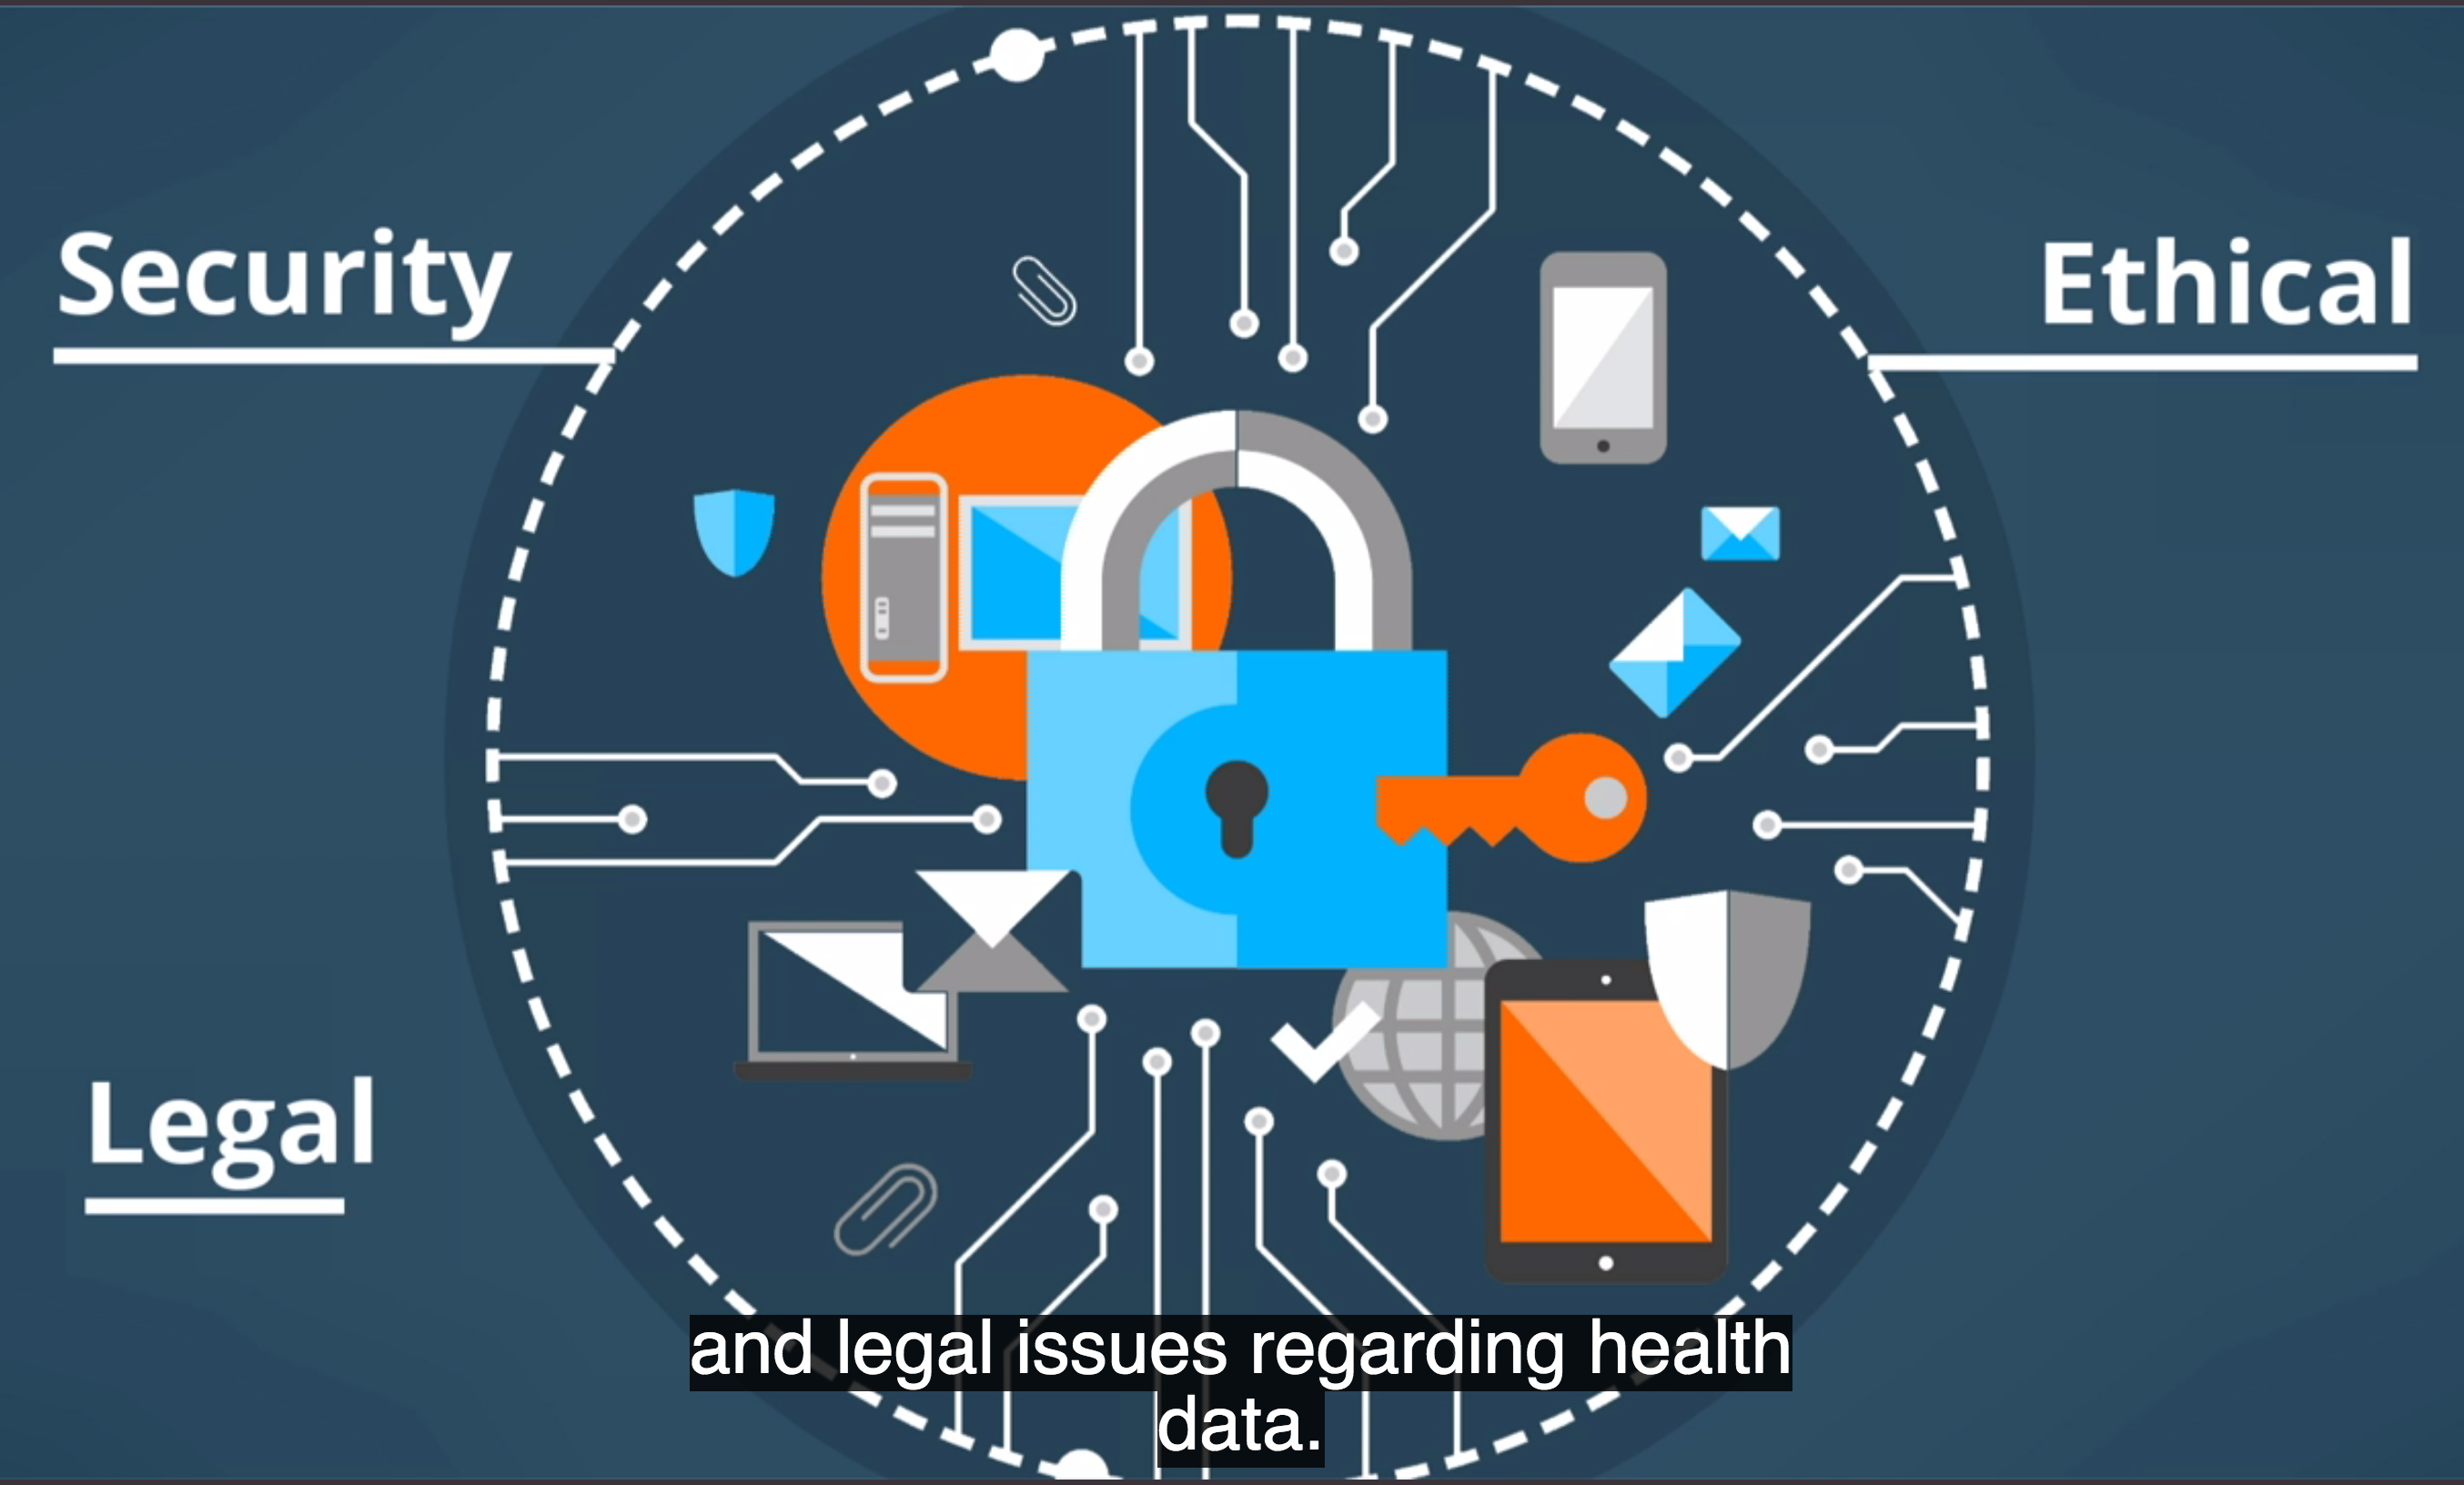
\includegraphics[width=\textwidth]{DataProtection_Issues.png}
         %\caption{}
         %\label{fig:}
     \end{subfigure}
     \hfill
%---------------------------------------------------%%
     \begin{subfigure}[b]{0.3\textwidth}
         \centering
         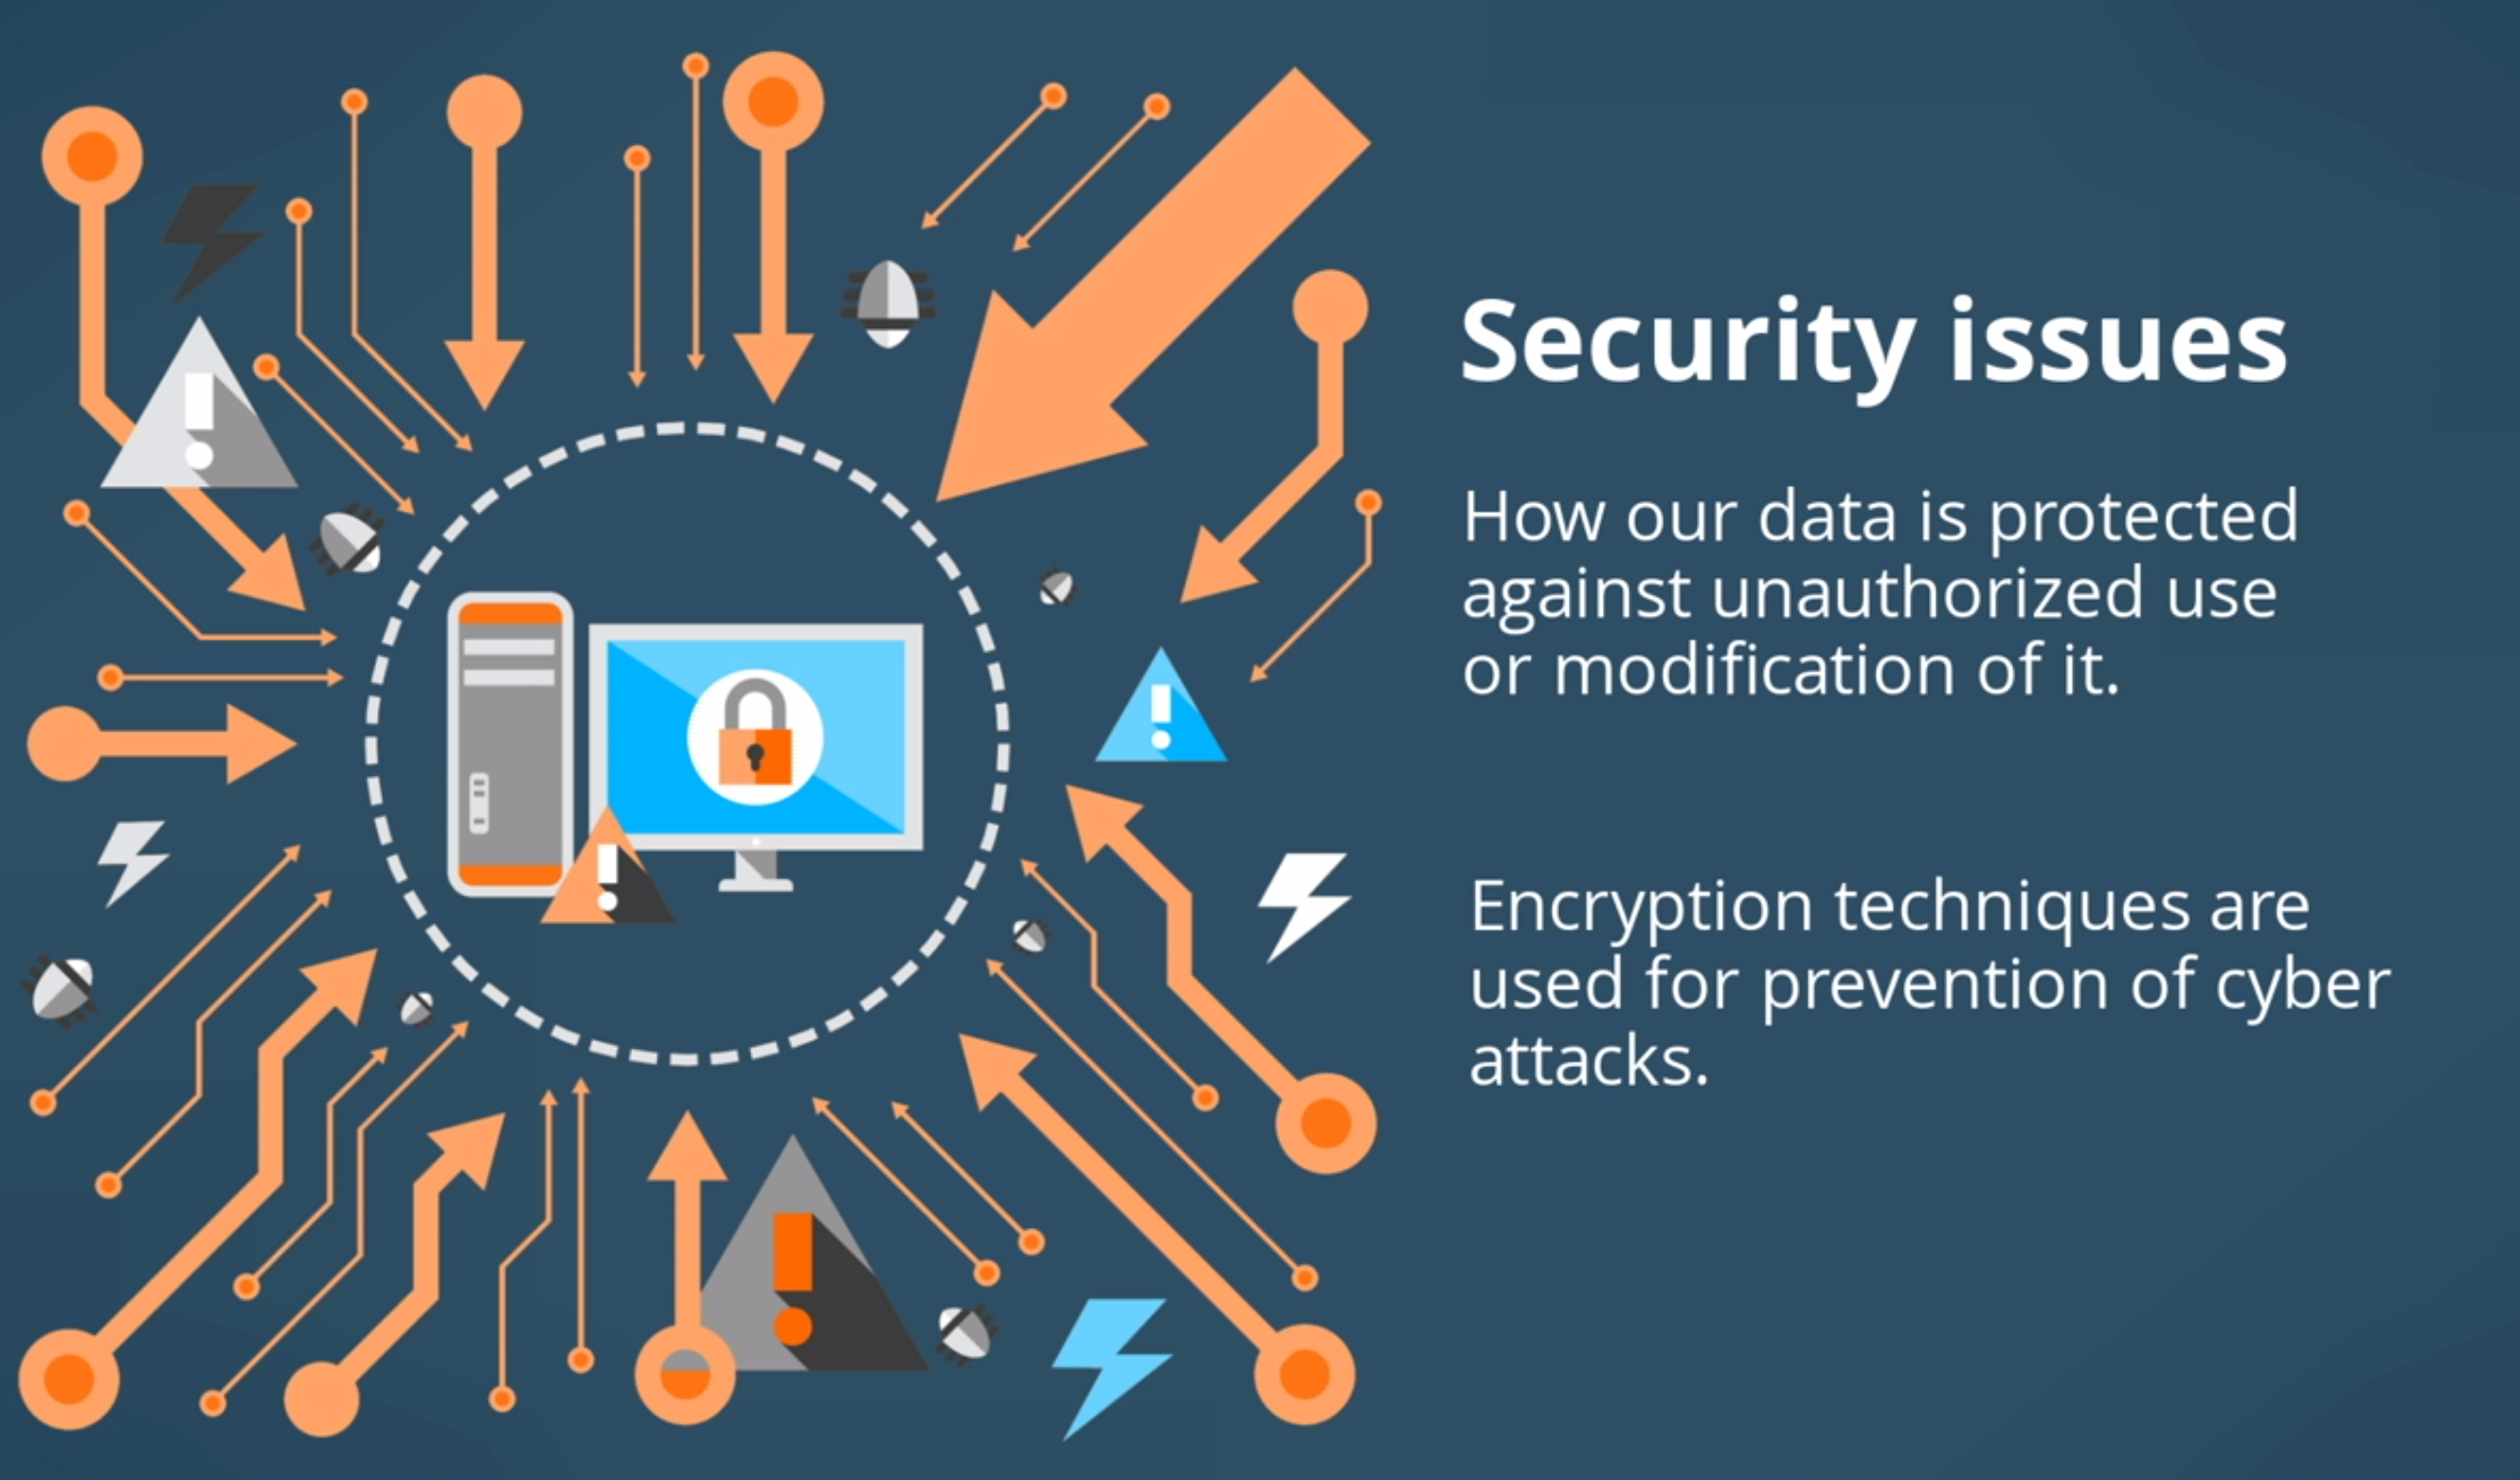
\includegraphics[width=\textwidth]{Security.png}
         %\caption{}
         %\label{fig:}
     \end{subfigure}
     \hfill
%---------------------------------------------------%%
\begin{subfigure}[b]{0.3\textwidth}
    \centering
    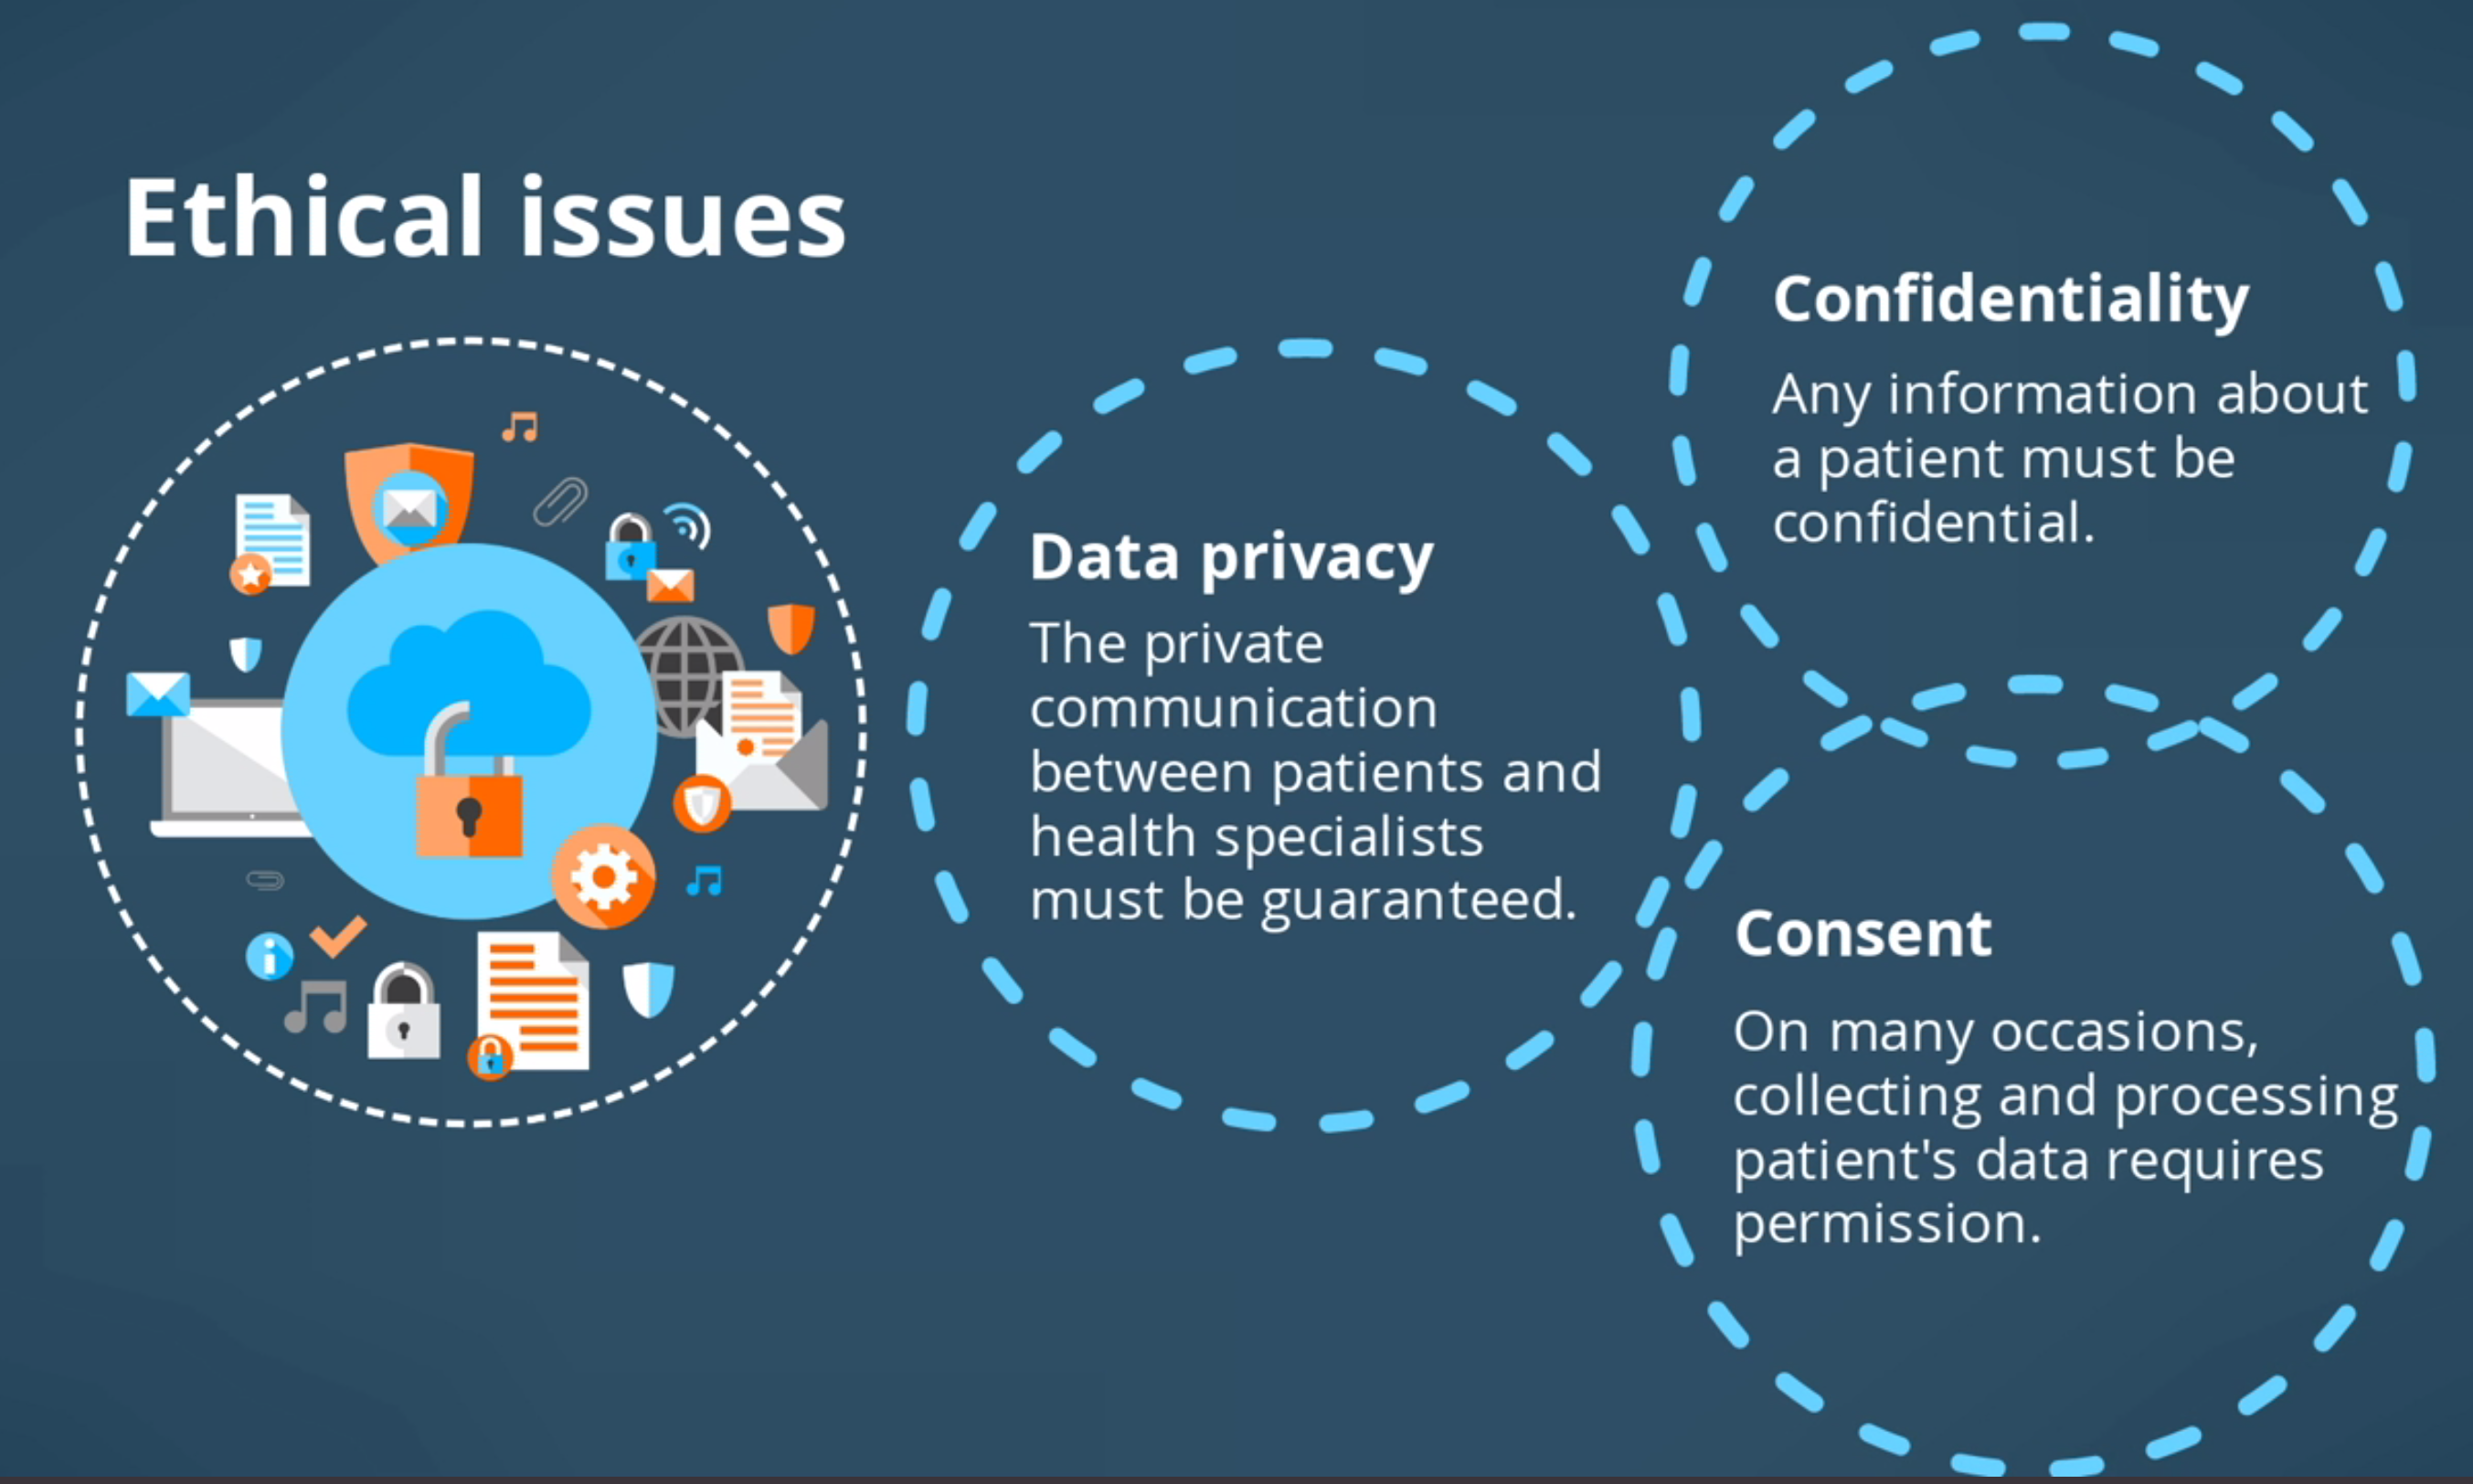
\includegraphics[width=\textwidth]{Ethics.png}
    %\caption{}
    %\label{fig:}
\end{subfigure}
\hfill
%---------------------------------------------------%%
\hfill
\\
{\scriptsize%
Source: \url{https://www.futurelearn.com/courses/managing-your-health-data/2/steps/473546}}
\caption{Data Protection Issues}
\label{fig:DataProtection_Issues}
\end{figure}
%---------------------------------------------------%%











%-------------------------------------------------------%
%-------------------------------------------------------%       
%-------------------------------------------------------%
%-------------------------------------------------------%                
\section{Read}
\renewcommand{\labelenumii}{\alph{enumii}}
      \begin{enumerate}
%-------------------------------------------------------%       
       \item  Electronic Health Records: Then, Now, and in the Future \url{https://www.ncbi.nlm.nih.gov/pmc/articles/PMC5171496/}
        \item   Overview of the national laws on electronic health records in the EU Member States \url{https://ec.europa.eu/health/ehealth/projects/nationallaws_electronichealthrecords_en/}
        \item  Gimme My DaM Data video from the American College of Medical Informatimusicology  \url{https://www.youtube.com/watch?v=0gpk-fbfg4Y&feature=youtu.be}   
        \item Plante and Colleagues Say High Ratings Don’t Mean Blood Pressure App Works \url{https://www.med.uvm.edu/com/news/2018/06/22/plante_and_colleagues_say_high_ratings_don_t_mean_blood_pressure_app_works}
        \item Health information on the Internet (Gold mine or minefield?) \url{https://www.ncbi.nlm.nih.gov/pmc/articles/PMC4020634/}
        \item The Global WannaCry cyber attack in May 2017 which targeted healthcare systems. \url{https://www.england.nhs.uk/wp-content/uploads/2018/02/lessons-learned-review-wannacry-ransomware-cyber-attack-cio-review.pdf}
 %-------------------------------------------------------%     

       \end {enumerate}   
 %-------------------------------------------------------%
%-------------------------------------------------------%
%-------------------------------------------------------%
%-------------------------------------------------------%                
\section{Resources}
\renewcommand{\labelenumii}{\alph{enumii}}
      \begin{enumerate}
%-------------------------------------------------------%       
       \item  WebMD  
           \begin{enumerate}
               \item \url{https://www.webmd.com/}
               \item a verified health information services website from the US
               \item The site publishes content relating to health, including a symptom checklist, drugs information and blogs from doctors who share their thoughts about specific topics. It also provides a means of storing personal medical information.
           \end{enumerate}
 %-------------------------------------------------------%     
       \item Medlineplus 
           \begin{enumerate}
               \item \url{https://medlineplus.gov/}
               \item MMedlineplus is written by health professionals but with content adapted to be accessed by patients.
               \item  It pulls together information from the US National Library of Medicine, National Institutes of Health and other US government agencies and healthcare organisations. 
               \item All the content is provided by clinical professionals.
               \item Optimised to be used on mobile devices, around 400 million people around the world have used the site. It can also use patient data within EHR systems and connect this data to related information on conditions and medications.
           \end{enumerate}
 %-------------------------------------------------------%     
       \item HealthVault 
           \begin{enumerate}
               \item Microsoft \url{https://international.healthvault.com/de/en}
               \item Can manage \textbf{Personal Health Record(PHR)} 
               \item \textbf{Entry all the data manually?! by the patients?!}
               \item The site allows individuals to share their entire health record or just selected data with others, such as doctors, healthcare professionals or relatives.
               \item It allows health and fitness data to be collected from selected devices like blood pressure monitors, heart rate watches and wifi bodyscales.
           \end{enumerate}
 %-------------------------------------------------------%     
       \item Google Fit Android App
           \begin{enumerate}
               \item Google and WHO \url{https://www.google.com/fit/}
               \item Movements management using accelerometer. 
               \item More moves, more heart points
           \end{enumerate}
 %-------------------------------------------------------%  
     \item  Qoolife
       \end {enumerate}   
%-------------------------------------------------------%
%-------------------------------------------------------%  
%-------------------------------------------------------%
%-------------------------------------------------------%     
\section{Questions}
\renewcommand{\labelenumii}{\alph{enumii}}
      \begin{enumerate}
%-------------------------------------------------------%      
       \item What health data is mainly used for?
          \begin{enumerate}  
              \item Clinical research
              \item Patient treatment (Electronic Health Records)
              \item Keep fit
           \end {enumerate}       
%-------------------------------------------------------%     
%-------------------------------------------------------%      
       \item The results obtained from a glucose blood tests are data or information?
          \begin{enumerate}  
              \item Data
              \item Information
           \end {enumerate}       
%-------------------------------------------------------%            
%-------------------------------------------------------%      
       \item The diagnosis “Diabetes” is data or information?
          \begin{enumerate}  
              \item Data
              \item Information
           \end {enumerate}       
%-------------------------------------------------------%      
%-------------------------------------------------------%      
       \item The Electronic Health Records use:
          \begin{enumerate}  
              \item Medical standards
              \item Clinical terminologies
              \item PC
              \item Mobile phones
           \end {enumerate}       
%-------------------------------------------------------%      
 %-------------------------------------------------------%      
       \item What are the benefits of using Electronic Prescriptions?
          \begin{enumerate}  
              \item Avoids duplicated prescriptions
              \item Periodic prescriptions for chronic patients
              \item No authentication is required
           \end {enumerate}       
%-------------------------------------------------------% 
 %-------------------------------------------------------%      
       \item Some wearable devices can:
          \begin{enumerate}  
              \item monitor different vital signs
              \item count steps
              \item track sleeping
           \end {enumerate}       
%-------------------------------------------------------% 
 %-------------------------------------------------------%      
       \item Which devices can be considered as Health Monitoring?
          \begin{enumerate}  
              \item Thermometer
              \item Blood pressure monitor
              \item Computer
           \end {enumerate}       
%-------------------------------------------------------% 
 %-------------------------------------------------------%      
       \item Why are some health monitoring devices used alongside mobile applications?
          \begin{enumerate}  
              \item To visualise your health data in your mobile
              \item Share health data with others
              \item It is more secure
              \item To store your health data in the cloud
           \end {enumerate}       
%-------------------------------------------------------% 




        \end {enumerate} 
  
 %-------------------------------------------------------%
%-------------------------------------------------------%
%-------------------------------------------------------%
%-------------------------------------------------------%       
\section{Answers}        
\renewcommand{\labelenumii}{\alph{enumii}}
      \begin{enumerate}
%-------------------------------------------------------%       
       \item What health data is mainly used for?
          \begin{enumerate}  
              \item Clinical research is based on the analysis of health data from multiple patients
              \item Patient treatment (frequently using EHRs) is the main way of generating and storing health data
           \end {enumerate}    
%-------------------------------------------------------%            
       \item The results obtained from a glucose blood tests are data or information?
          \begin{enumerate}  
              \item Clinical research is based on the analysis of health data from multiple patients
              \item Patient treatment (frequently using EHRs) is the main way of generating and storing health data
           \end {enumerate}       
%-------------------------------------------------------%            
%-------------------------------------------------------%      
       \item The diagnosis “Diabetes” is data or information?
          \begin{enumerate}  
              \item Diabetes is a diagnosis provided by a doctor based on symptoms and results from a laboratory test, it is therefore Information.
           \end {enumerate}       
%-------------------------------------------------------%      
 %-------------------------------------------------------%      
       \item The Electronic Health Records use:
          \begin{enumerate}  
              \item To facilitate appropriate analysis of data, EHR systems need to use standards in medicine to be homogeneous across regions and systems\
              \item Terminologies like the International Classification of Diseases (ICD) by the World Health Organization are generally used to store your health data in an EHR
           \end {enumerate}       
%-------------------------------------------------------% 
 %-------------------------------------------------------%      
       \item What are the benefits of using Electronic Prescriptions?
          \begin{enumerate}  
              \item Typos, duplicates and other mistakes associated with paper records can be avoided when data is stored in an electronic form; potentially avoiding life threatening problems.
              \item When patients need to be dispensed the same drug periodically, e-prescription can help facilitate this process and save time for health professionals and patients.
           \end {enumerate}       
%-------------------------------------------------------% 
 %-------------------------------------------------------%      
       \item Some wearable devices can:
          \begin{enumerate}  
              \item Wearables are electronic devices that can be embedded into clothes or worn as accessories. Modern smartwatches can measure heart rate, for example.
              \item Mobile phones or smartwatches include GPS. Taking into account speed and distance, they can estimate the number of steps you take.
              \item If worn during the night, some devices can estimate periods and levels of sleep.
           \end {enumerate}       
%-------------------------------------------------------% 
 %-------------------------------------------------------%      
       \item Which devices can be considered as Health Monitoring?
          \begin{enumerate}  
              \item Devices with a sensor to measure the temperature and a display to show the numerical value are very common to check if we have fever.
             \item Blood pressure is an important vital sign measuring the pressure on the wall of vessels that can be monitored with devices at home
           \end {enumerate}       
%-------------------------------------------------------% 
       \item Why are some health monitoring devices used alongside mobile applications?
          \begin{enumerate}  
              \item Mobile displays are usually better than wearables with built-in displays, as they are able to show the gathered data
              \item Since mobile phones are generally connected to the internet, we can upload the corresponding data to the cloud and share it with other users.
              \item Connecting to a mobile facilitate sharing of your health data, but there are more opportunities to share the data with undesired people, so it is in fact more insecure
              \item With data uploaded to the cloud, we can store it for future consultation or gather it from different applications and devices.
           \end {enumerate}       
%-------------------------------------------------------% 

\end {enumerate} 
 %-------------------------------------------------------%
 
 
 
%-------------------------------------------------------%
%-------------------------------------------------------%
%-------------------------------------------------------%
\section{Think}
\renewcommand{\labelenumii}{\alph{enumii}}
      \begin{enumerate}
%-------------------------------------------------------%       
       \item  What is the difference between EHR and e-prescription?
        \item  What is the the importance of health data security?
        \item What are the technological barriers of managing our health information today?
        \item What are your main concerns on privacy related to your health data?
        \item What are the consequences to giving citizens more control over their own data? Or do you think that it will disconnect people from healthcare professionals?
        \item How do you plan to change your behaviour in regards to managing your personal health and activity data?

      \end {enumerate}
%-------------------------------------------------------%
%-------------------------------------------------------%
%-------------------------------------------------------%
%-------------------------------------------------------%   
\section{Survey}
%-------------------------------------------------------%
%insert a figure
    \begin{figure}[H]
      \centering
      \stackunder{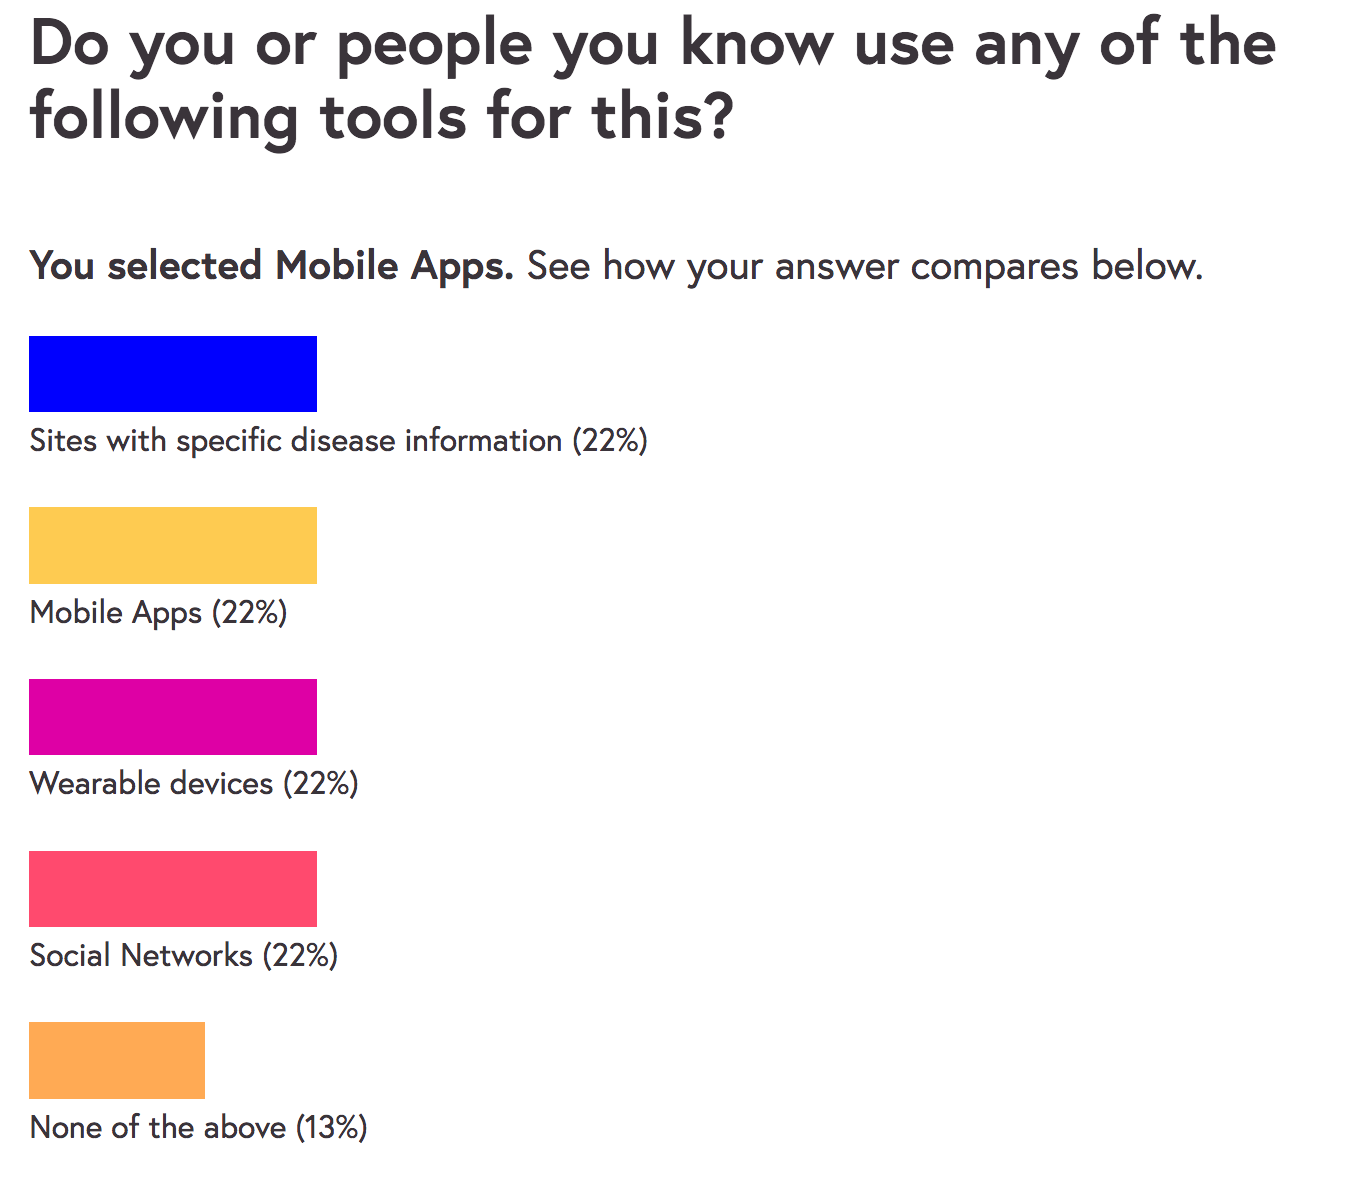
\includegraphics[width=0.6\textwidth]{Infor_survey.png}}%
            {\scriptsize%
            Source: \url{https://www.futurelearn.com/courses/managing-your-health-data/2/steps/473553}}
 \caption{Do you or people you know use any of the following tools for this?}
 %\label{fig:Infor_survey}
 \end{figure}
    %end of a figure
%-------------------------------------------------------%
%-------------------------------------------------------%
%insert a figure
    \begin{figure}[H]
      \centering
      \stackunder{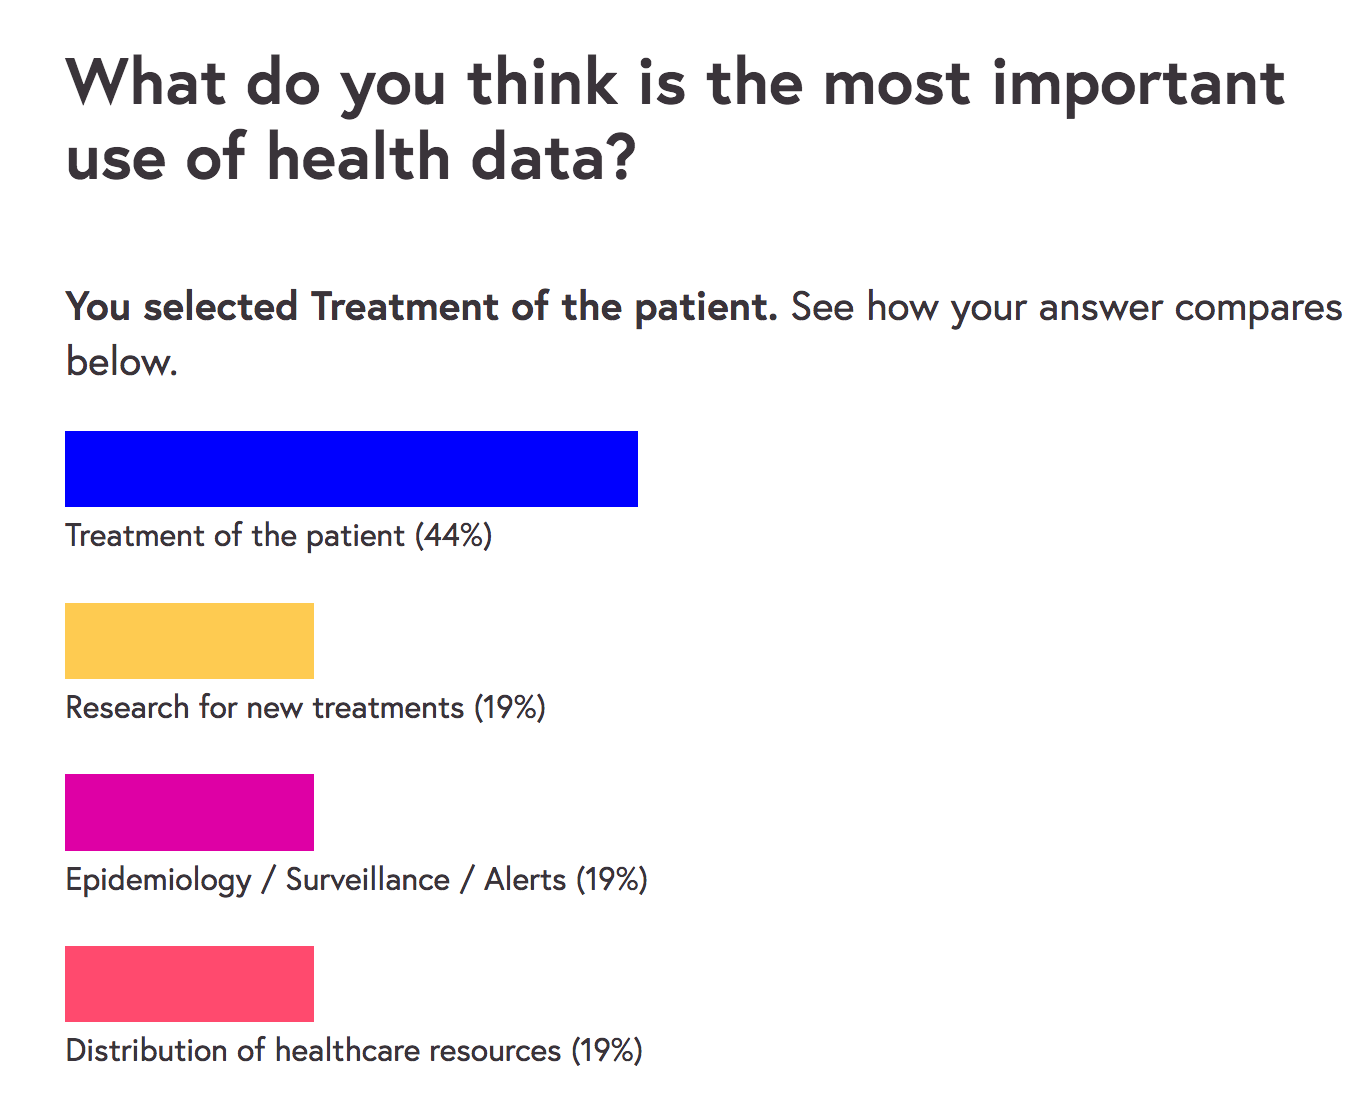
\includegraphics[width=0.6\textwidth]{use_health_data.png}}%
            {\scriptsize%
            Source: \url{https://www.futurelearn.com/courses/managing-your-health-data/2/steps/473567}}
 \caption{What do you think is the most important use of health data?}
 %\label{fig:Infor_survey}
 \end{figure}
    %end of a figure
%-------------------------------------------------------%
%-------------------------------------------------------%
%insert a figure
    \begin{figure}[H]
      \centering
      \stackunder{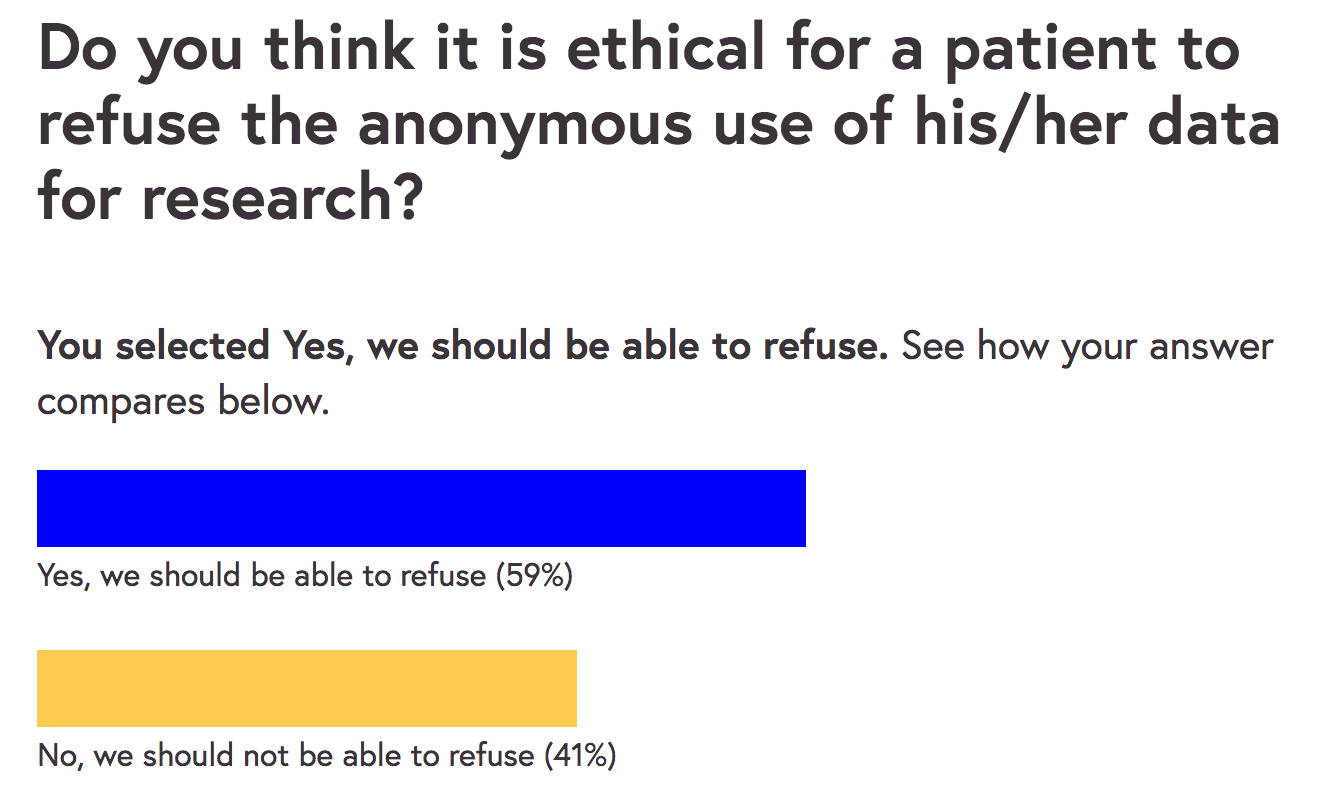
\includegraphics[width=0.6\textwidth]{Refuse_use.png}}%
            {\scriptsize%
            Source: \url{https://www.futurelearn.com/courses/managing-your-health-data/2/steps/473568}}
 \caption{Is it ethical for a patient to refuse the anonymous use of his/her data for research?}
 %\label{fig:Infor_survey}
 \end{figure}
    %end of a figure
%-------------------------------------------------------%

%-------------------------------------------------------%
%insert a figure
    \begin{figure}[H]
      \centering
      \stackunder{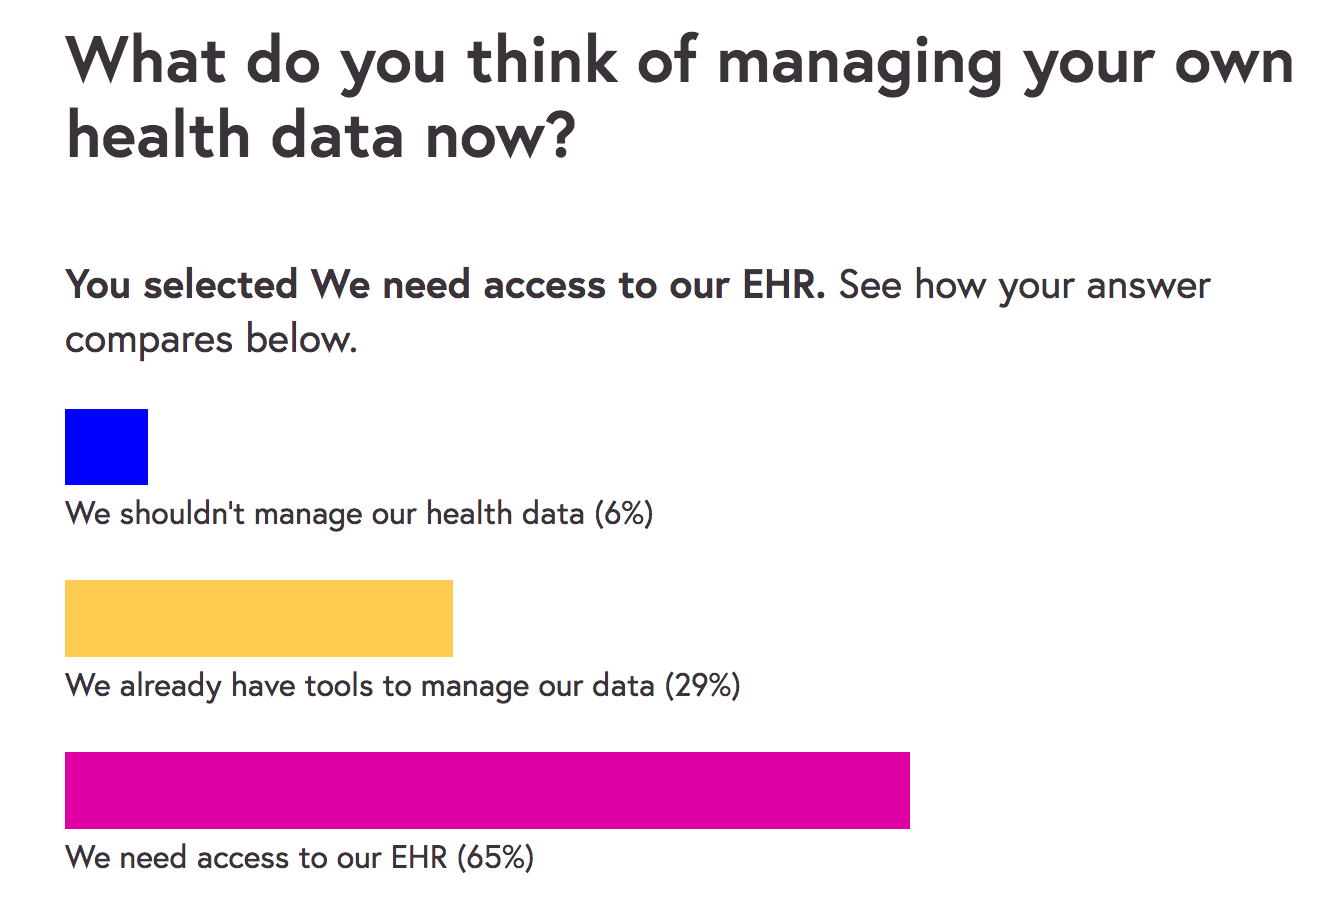
\includegraphics[width=0.6\textwidth]{Magage_data.png}}%
            {\scriptsize%
            Source: \url{https://www.futurelearn.com/courses/managing-your-health-data/2/steps/473560}}
 \caption{What do you think of managing your own health data?}
 %\label{fig:Infor_survey}
 \end{figure}
    %end of a figure
%-------------------------------------------------------%
%Congratulations, you have reached the end of this course! Well done for all your hard work.
% Well, it was not hard. A bit oversimplified.

\end{document}